\documentclass[12pt]{article}

\usepackage[margin=0.5in, includefoot]{geometry}
\usepackage{setspace}
\usepackage{titlesec}
    \titleformat{\subsubsection}{\normalfont\normalsize\itshape}{\thesubsubsection}{1em}{}
\usepackage{hyperref}
\usepackage{xurl} % yay this works
    \hypersetup{
        colorlinks=true, 
        linkcolor=blue, % can comment this out if the blue figure faces is bothersome
        urlcolor=cyan
    }
    \renewcommand{\figureautorefname}{\textbf{Figure}} % decent fix but later should figure out how to make numbers bolded too
\usepackage{enumitem}
    \setlist[enumerate]{label=(\arabic*)}
\usepackage{amsmath}
\usepackage{amssymb} % for mathfrak font style
\usepackage{mathrsfs} % for mathscr font style
\usepackage{bm}
\usepackage{physics}
\usepackage{cancel}
\usepackage{xfrac}
\usepackage{array}
\usepackage{multicol}
\usepackage{float}
\usepackage[many]{tcolorbox}
    \definecolor{cellborder}{HTML}{CFCFCF}
    \definecolor{cellbackground}{HTML}{F7F7F7}
\usepackage{listings}
    \lstset{
        basicstyle=\scriptsize\ttfamily, % font style
        escapeinside={(*@}{@*)} % escape into LaTeX using (*@ and @*)
    }
\usepackage{subcaption}
\usepackage{wrapfig}
\usepackage{graphicx}
\usepackage{multirow}
\usepackage{csvsimple}
\usepackage[font=small]{caption}
\usepackage{xcolor} % for formatting purposes
\usepackage{lipsum} % for formatting purposes
% \usepackage[hang, flushmargin]{footmisc} % seeing if default setup is actually nice looking

\renewcommand{\thesubsection}{\arabic{subsection}}
\newcommand{\totder}[2][]{\frac{\mathrm{d}#1}{\mathrm{d}#2}} % needs amsmath package
\newcommand{\parder}[2][]{\frac{\mathrm{\partial#1}}{\mathrm{\partial#2}}} % needs amsmath package
\newcommand{\diff}[1]{\mathrm{d}#1}

\renewcommand{\Re}{\mathfrak{Re}} % these are just cooler
\renewcommand{\Im}{\mathfrak{Im}}
\newcommand{\im}{\mathrm{i}}
\newcommand{\R}{\mathbb{R}}

\newsavebox\foobox
\newlength{\foodim}
\newcommand{\slantbox}[2][0]{\mbox{%
        \sbox{\foobox}{#2}%
        \foodim=#1\wd\foobox
        \hskip \wd\foobox
        \hskip -0.5\foodim
        \pdfsave
        \pdfsetmatrix{1 0 #1 1}%
        \llap{\usebox{\foobox}}%
        \pdfrestore
        \hskip 0.5\foodim
}}
\def\Lagrangian{\slantbox[-0.2]{$\mathcal{L}$}} % ok wow nailed it (I think?)
\def\Fourier{\slantbox[-0.45]{$\mathscr{F}$}} % kinda legible yeah

\begin{document}
\setstretch{1.15}

\section*{Peak Analysis, Source Identification, and Gaussian Curve Fitting for Gamma Ray Spectroscopy}

\begin{quote}
    Jeff Lam, Ana McKiernan \\
    \textit{Department of Physics, Binghamton University} \\
    May 12\textsuperscript{th}, 2025
\end{quote}

\subsection*{Abstract}
Gamma ray spectra for the radioactive sources Cs-137, Co-60, an unknown sample,
and Na-22 were constructed using data collected from a scintillation detector.
Scintillation materials luminesce under the presence of radioactivity, a consequence
of the theories behind various modern physics phenomena, such as the photoelectric
effect and Compton scattering. The specific scintillation detector used for gamma ray
spectroscopy consisted of a thallium-doped sodium iodide (NaI(TL)) crystal hermetically sealed as a 
base, a photomultiplier tube to convert light from photoevents as weak signal to high-voltage outputs, and a 
digibase controller to organize each output into ``channels''--- histogram bins that represent different orders of 
energy levels. Various categorical peaks were considered, mainly the typical photopeaks amongst others
such as backscatters, Compton edges, and annihilation. After developing Python code to help
identify the appropriate channel number corresponding to the location of each photopeaks,
a calibration curve was fitted using weighted linear-least squares fitting when
additionally given the known energy levels of these photopeaks for Cs-137 and Co-60.
The result is a calibration curve of the form $\hat{y}=0.1759x+12.6326$, allowing the performance
of more advance experimental procedures on radiation sample. The first use case involved
identifying an unlabeled radiation sample, which was successfully identified as Sb-125
using the same code that helped ascertain photopeak position channel number, and the second use case
involved some success in fitting Gaussian curves to various explainable peaks of Na-22,
to which the qualitative goodness in its fit can be seen and accessed.

\noindent\rule{\linewidth}{0.5pt}

\begin{multicols}{2}

\subsection{Introduction}
Radiation detectors are used to determine the presence of radioactive materials
and for possible identification of said material. Typically, isotopes of various 
heavy elements are the sources of radioactive materials, where the amount of
the isotopes present is generally of interest. These ``nuclear material''
emits gamma radiation of typically a few hundred keV or less, X-rays via
beta decay, and alpha radiation via alpha decay [\hyperref[sec:1]{1}].
\vfill

\subsubsection{Gamma Ray Spectroscopy}
The gamma ray radiation emitted by nuclear materials are characteristic of the
source element, allowing the identification of the isotopes. Various instruments
may be used to detect gamma ray radiation such as gas filled detectors, 
scintillation detectors, semiconductor detectors, \textit{etc}. Of these,
scintillation and semiconductor detectors are the most extensive, however 
they suffer setbacks including but not limited to being operable only for 
small radioactive samples and lower efficiency [\hyperref[sec:2]{2}]. 
The experiments involved in this paper employ a scintillation detector
for detecting these radiation signals---
refer to section \textit{3.1 Scintillation Detectors} for the working
theories behind scintillation and section \textit{3.2 Apparatus} for
the model and brand type used for the experiments.

\subsection{Theory}

There are three interactions that may occur 
within a scintillation material when gamma rays pass 
through: the photoelectric effect, Compton scattering,
and annihilation due to pair production.
There are also X-ray emissions that occurs as a result
of (primarily) the photoelectric effect.
Of the three events, the first two are nearly ubiquitous
across all radioactive materials---
annihilation may be seen in one of the samples where
data was collected in this paper, Sodium-22 (Na-22).

\subsubsection{The Photoelectric Effect}
\textbf{Figure 1} showcases the underlying principle behind
the photoelectric effect. As it can be seen, an incoming photon
interacts with a bound electron within the $K$-shell,
transferring nearly all of its energy to the particle,
thereby becoming a photoelectron by breaking the binding
energy tied to its orbit around the atom. Let $E_\gamma$ be the
energy of the incident ray, $E_\text{bind.}$ be the binding energy
of the target electron, and $E_e$ be the energy of the photoelectron.
Because of the nearly complete transfer of energy from the photon to
the electron, the Law of Conservation of Energy may be applied to produce the
equation
$$E_e=E_\gamma-E_\text{bind.}$$
If the bound electron's binding energy is small (\textit{i.e.}, electrons
orbiting with the $K$-shell of its atom), then all kinetic energy carried
by the photon is converted to the photoelectron, \textit{i.e.}, $E_\text{bind.}$
is negligible.

For the bound electron knocked out of orbit that
\begin{figure}[H]
    \centering
    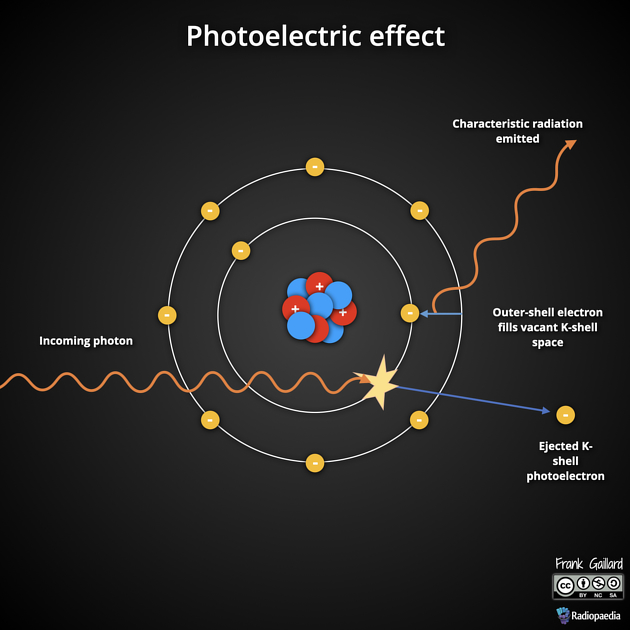
\includegraphics[width=0.98\linewidth]{figs/fig1.jpeg}
    \caption{
        References diagram on the photoelectric effect [\hyperref[sec:3]{3}]
    }
\end{figure}
\noindent
was turned into a photoelectron,
a neighboring electron orbiting within the next energy level, the $L$-shell, may
replace the lost electron at its position, releasing some of the energy that
it held when orbiting at the larger shell. These emissions are typically within
the X-ray range, hence the term \textit{X-ray emissions}. For certain radioactive
isotopes, peaks picked up within the lower energy range may likely be these X-ray
emissions.

\subsubsection{Compton Scattering}
\textbf{Figure 2} showcases an alternative interaction that may occur within
scintillation: Compton scattering. In this scenario, a photon interacts with
an electron in orbit of its parent atom, but unlike the photoelectric effect,
its energy is not completely transferred over to create a photoelectron---
instead, a recoil electron is produced, and the rest of the photon energy
scatters away at some angle $\theta$ from the recoil electron.
In this scenario, $E_\gamma$ only loses a portion of its kinetic energy---
let $E_\gamma'$ be the final kinetic energy carried by the scattering photon.
The energy relationship between the two can be written as
$$E_\gamma'=\frac{E_\gamma}{1+1.96\;\mathrm{MeV}E_\gamma\big(1-\cos(\theta)\big)}$$
A derivation of this surprising result can be seen in \textbf{Appendix A: Derivation of the Compton Scattering Formula},
attached at the end of this paper.

For the special case that $\theta=\frac{\pi}{2}$, $\cos(\theta)=-1$, and so the
relationship can be further simplified to
$$E_\gamma'=\frac{E_\gamma}{1+3.91\;\mathrm{MeV}E_\gamma}$$
Geometrically, this special case represents the scenario where both the scattering
photon ray and recoil electron scatters antiparallel to each other. This interaction
is therefore dubbed as ``backscatter''\textsuperscript{$\dagger$},
and is yet another spectral feature that manifest as a peak during gamma ray spectroscopy.
\renewcommand{\thefootnote}{$\dagger$}
\footnotetext{
    This, Compton scattering, and the photoelectric effect can be considered analagous
    to some classical mechanics interaction involving games of pool,
    for the various scenarios and results of a cue ball hitting an 8-ball from various
    conditions. For those familiar with pool/billiards terminology involving shot types,
    the backscatter interaction may be compared to a ``draw shot'',
    the Compton scattering compared to an angled shot,
    and the photoelectric effect compared to the ``stopped shot''.
}
\begin{figure}[H]
    \centering
    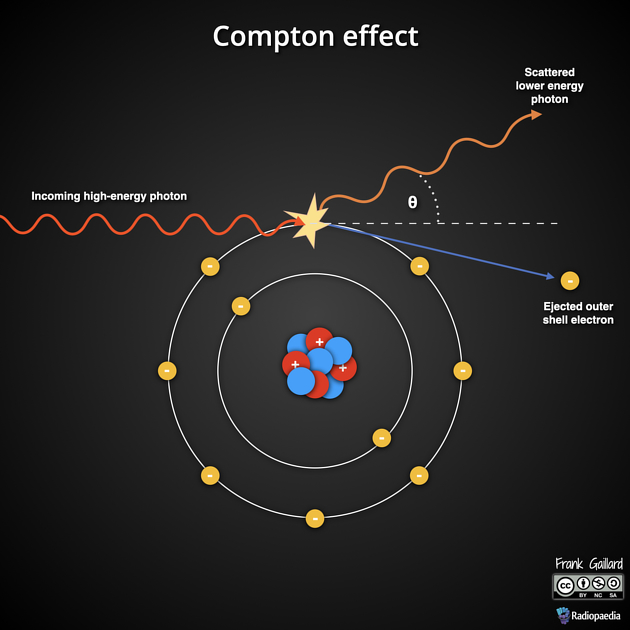
\includegraphics[width=0.98\linewidth]{figs/fig2.jpeg}
    \caption{
        References diagram on the Compton effect [\hyperref[sec:4]{4}]
    }
\end{figure}
\begin{figure}[H]
    \centering
    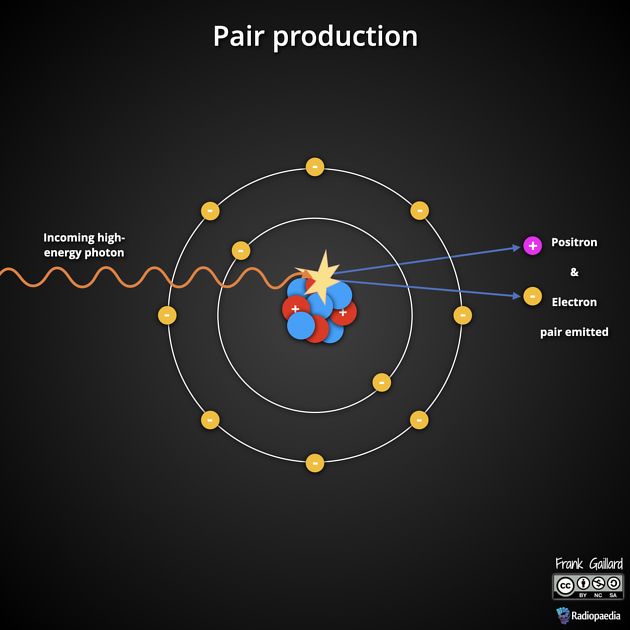
\includegraphics[width=0.98\linewidth]{figs/fig3.jpeg}
    \caption{
        References diagram on pair production and annihilation [\hyperref[sec:5]{5}]
    }
\end{figure}
\noindent
\subsubsection{Pair Production and Annihilation}
\textbf{Figure 3} showcases one more scenario that may occur when gamma rays
passes through (specifically) matter. If a gamma ray holding a kinetic energy
at least greater than or equal to twice of that of an electron's resting energy
($\approx511\;\mathrm{keV}$), and if the ray passes through the nucleus of an atom,
then it may convert into an electron, or more formally a \textit{beta particle}
($\beta^-$). But according to the Law of Conservation of Energy and Conservation
of Momentum, an \textit{anti-particle} is also created, holding the same but opposite
charge of the electron and scattering at an equal angle opposite of the normal
between it and the propogating beta particle. This anti-particle is dubbed the
\textit{positron} ($\beta^+$).

Though the produced beta particle ($\gamma\rightarrow\beta^-+\beta^+$)
scatters away from the interaction, the positron being anti-matter nearly always
interact with a neighboring electron, annihilating each other (hence the term
``annihilation'') and producing two other gamma rays that scatters opposite of
each other as well.

\subsection{Methods}
\subsubsection{Scintillation Detectors}
Scintillation detectors rely on scintillation materials---
materials that luminesce under the presence of high-energy rays 
near the X-ray portion of the electromagnetic spectrum.
Every gamma ray that passes through scintillation materials produces a light pulse,
and each light pulse can be thought of as an individual ``event'',
thereby producing signals that may be processed.
These signals, however, by themselves are too weak to be detected,
and so in order to properly detect them a process called photomultiplication helps
amplify these signals as high voltage outputs. 
These high voltage outputs then may be digitally logged by a computer software
\begin{figure}[H]
    \centering
    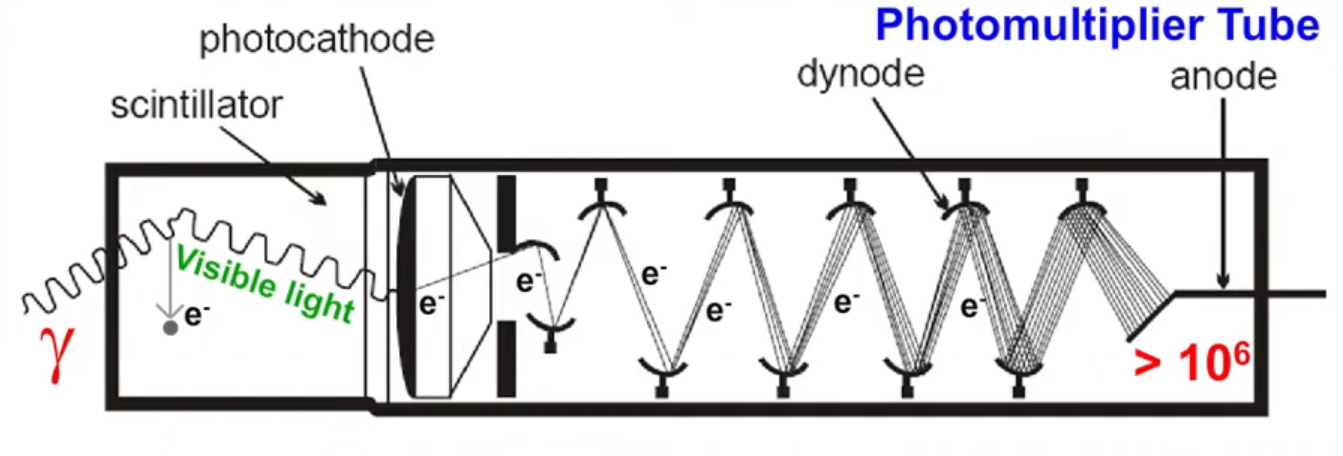
\includegraphics[width=0.98\linewidth]{figs/fig4.png}
    \caption{
        Snipped screenshot of [\hyperref[sec:6]{6}] showcasing the
        process of photomultiplication.
    }
\end{figure}
\noindent
\textbf{Figure 4} is a snipped screenshot of
a reference, showcasing the steps of photomultiplication.
Photomultiplication takes place in a PhotoMultiplier 
Tube (PMT), where the mechanism of the process is 
done. Incident radiation interacts with electrons 
within the scintillating materials, allowing for the 
events as mentioned in sections \textcolor{red}{1.2} and \textcolor{red}{1.3} to occur. 
The resulting photon is released as visible light and 
then enters a photocathode, where electrons 
proportional to the number of photons entered are 
released. Sets of High-Voltage (HV) dynodes then
amplify these
\begin{figure}[H]
    \centering
    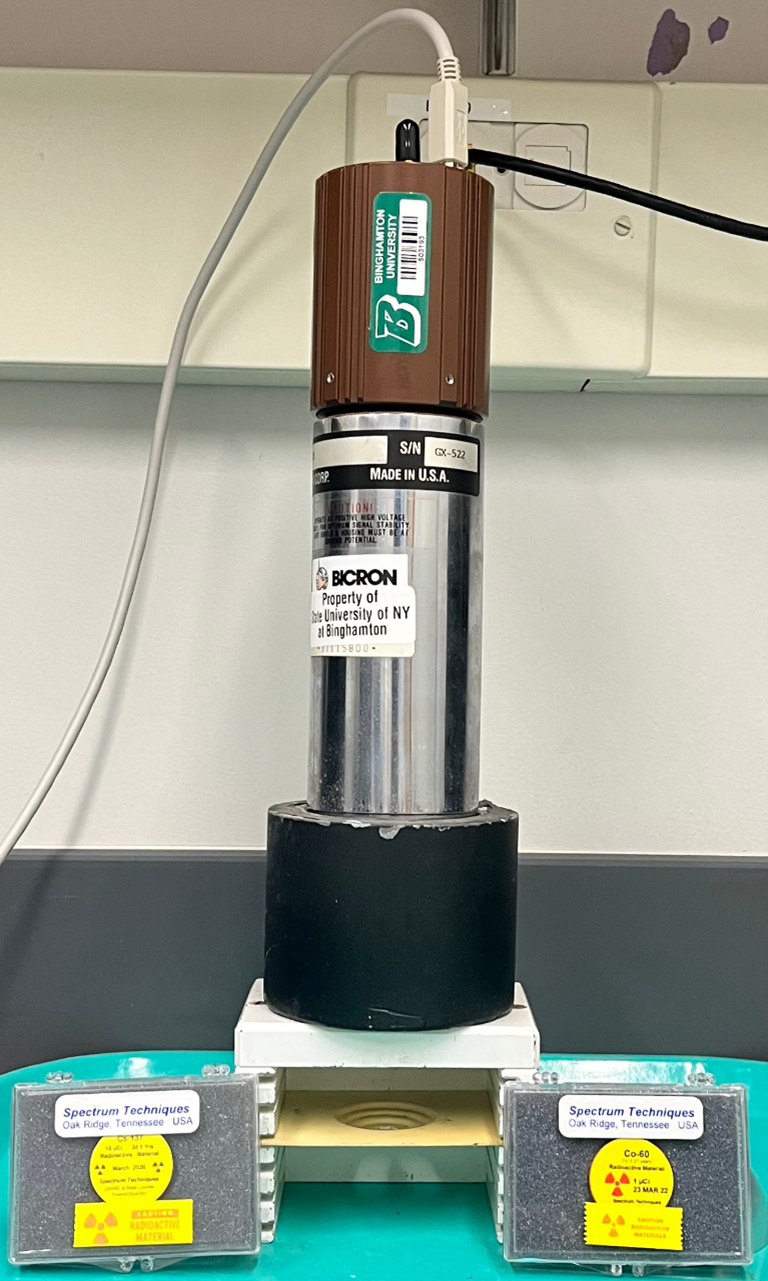
\includegraphics[width=0.98\linewidth]{figs/fig5.png}
    \caption{
        Image of the scintillation detector used for 
        gamma ray spectroscopy. Present are two radiation 
        sources, isotopes Cs-137 and Co-60, by the detector, 
        which is also coupled with a lead shield and a base to set 
        the radioactive materials. 
    }
\end{figure}
\noindent
electrons via secondary emissions. By 
the end, an anode picks up a voltage source that has 
more than a million more electrons than the original 
signal [\textcolor{red}{7}]. 

\subsubsection{Apparatus}
\textbf{Figure 5} is an image of the scintillation 
detector used for the gamma ray spectroscopy. A 2 in.
by 2 in. thallium-doped (TL) sodium iodide (NaI) crystal
(\textit{a.k.a.}, NaI(TL)) act as the detector's base,
hermetically sealed to prevent damage since  NaI (TL) is
hydroscopic. The base of the detector can be seen shrouded
by a lead shield, protecting the crystal from sending signals
from background radiation. 

The cylindrical metal tube on top of the base  is the PMT. 
The last component is an ORTEC digibase controller, an electronic
component that contains an HV source, amplifier, Pulse Height Analyzer
(PHA), and a digital MultiChannel Analyzer (MCA). This setup
essentially allows light signals from a radiation source to be picked
up after photomultiplication, counting them into ``channels''.
These channels are the energy levels that the device bins them in,
so a gamma ray spectrum of a radioactive isotope is essentially a 
histogram.

\subsubsection{Object}
The explanation of the mechanics behind the 
scintillation detector exposes then the objective of 
this experiment, which is to calibrate these channels 
into energy units so a calibration curve may be 
constructed and therefore be used to experimentally 
identify any photopeaks amongst other within a gamma ray 
spectrum. 

The digibase, in what is called a conversion 
gain, has two adjustable settings: a course gain and a 
fine gain. The course gain is actually the set channels 
that the device bins the counts of photoevents in---
it cannot be adjusted through the provided MAESTRO software
in the laboratory. Adjusting the course gain can only be
achieved by physically dismantling the digibase and changing an 
internal switch within its electronics. For the purpose 
of this experiment, the default setting of the course 
gain was left as is, which sets the spectrum to 1024 
channels. The fine gain setting is accessible to MAESTRO,
allows shifting of the channels to specific energy levels---
The procedure regarding the extensive adjustment of this setting is 
explained more in the next section.

\subsubsection{General Procedure}
With the digibase connected to a Radiation 
Lab computer via USB-B cable, the MAESTRO software 
that was already downloaded and present within the 
laboratory computer was opened. 
From the menu, the MCA settings were accessed, and 
first the HV setting was set to a range of 800V-900V. 
The fine gain under the amplifier tab of the setting 
was initially set to 1.0 as a benchmark, but ultimately
was kept for the rest of the experiments featured in this paper.

A radiation source may be placed on top of the panel inserted in a 
shelf level as seen in \textbf{Figure 5}. MAESTRO software provides
basic spectroscopy feature such as searches for Regions of Interests (ROI),
changes in window width, \textit{etc}., but ultimately the software was used
to just collect the count data amongst the 1024 channels for later analysis in
Python. Generally, data collection lasted for approximately one hour for each
experiment unless otherwise specified by the lab manual. For data exporting,
MAESTRO supports several formats, none which however are typical standard
file extensions (\textit{e.g.}, \texttt{.csv}. \texttt{.xlsx}, \textit{etc.})
Out of all possible file extensions offered, \texttt{.spe} was found to be
openable as a plain \texttt{.txt} file, so it was settled as the file extension
to export the data.

\subsection{Data Analysis}
All code written to produce graphs and perform data analysis can be found within
\textbf{Appendix B: Full Code Written for Analysis}.

\subsubsection{Source Distance on Resolution}
\textbf{Figure 6} shows an overlaid spectroscopy graph of various data gathered on
Cobalt-60 (Co-60) for a given shelf level underneath the scintillator.
It can be considered reasonable to guess that for equal time lapses of 1 hr
for data collection, the distance between the radiation source and the scintillator
is
\end{multicols}
\begin{figure}[H]
    \centering
    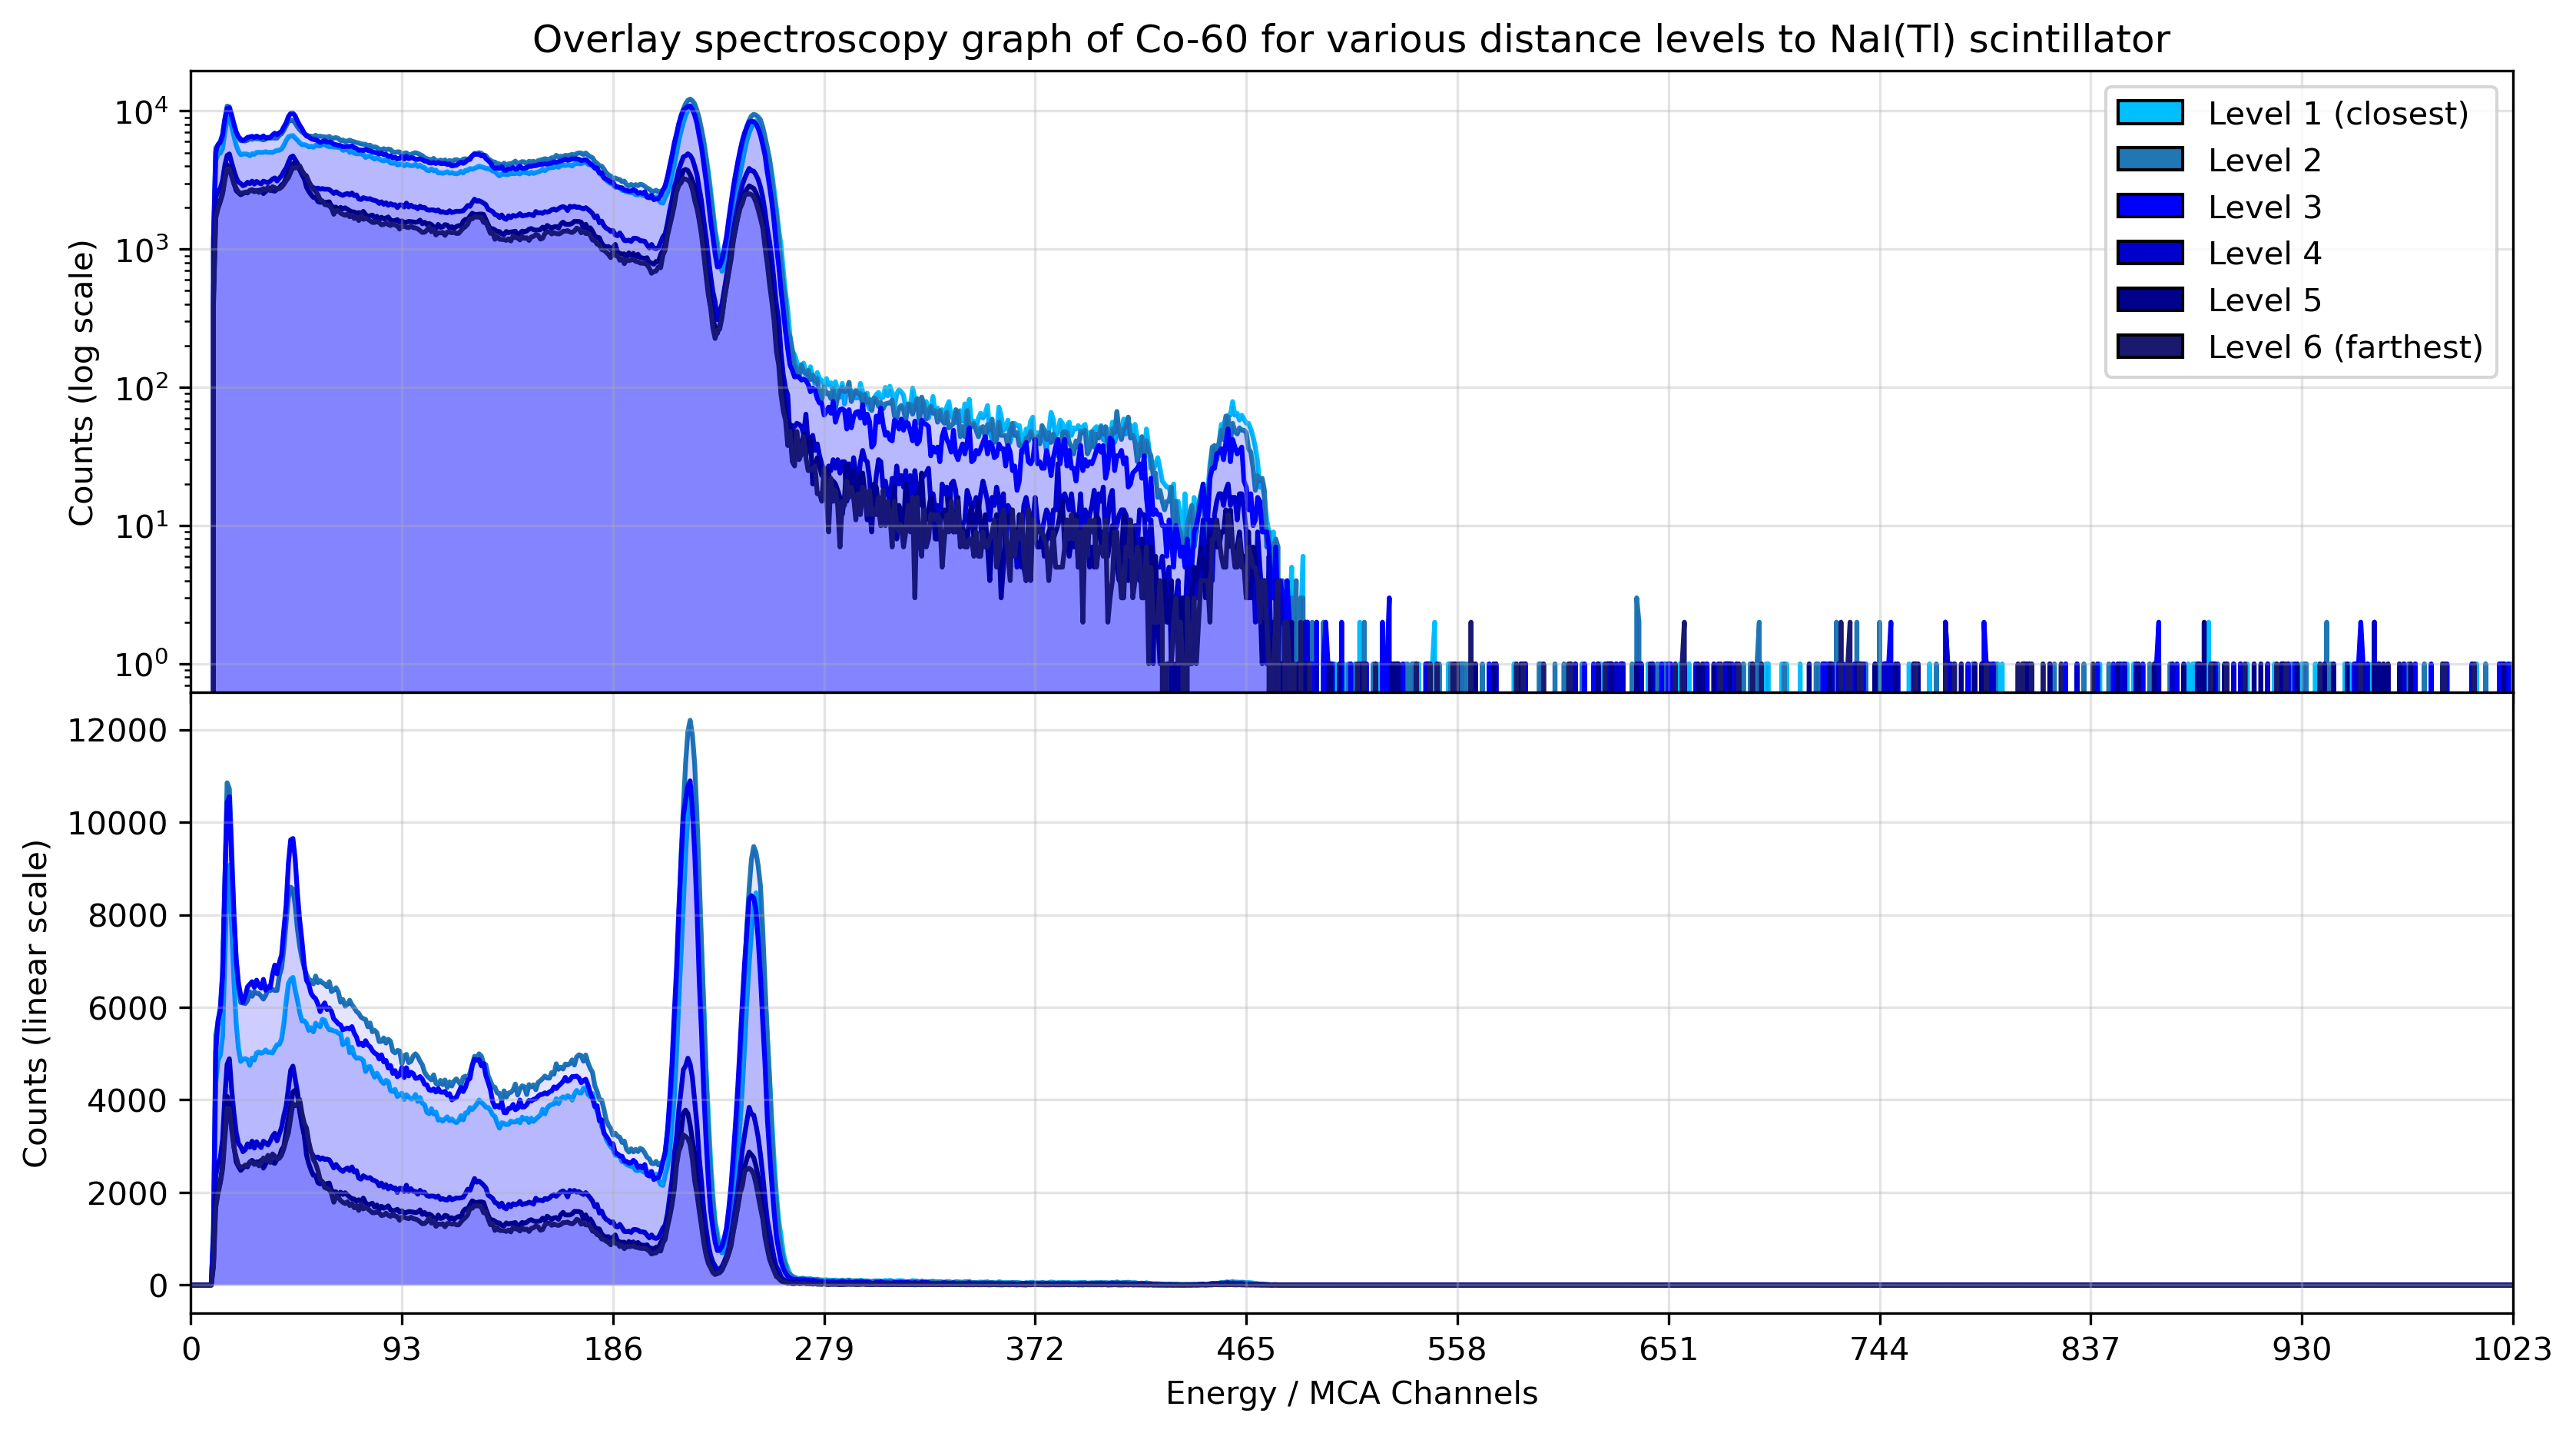
\includegraphics[width=0.98\linewidth]{figs/fig6.png}
    \caption{
        Overlay gamma ray spectroscopy of 6 different data gathering on source distance.
    }
\end{figure}
\begin{multicols}{2}
\noindent
inversely proportional to the counts obtained (\textit{i.e.}, the farther away
the sample is, the less event that can be detected by the scintillator).
However, it can be seen that \textbf{Figure 6} does not follow that ansatz,
though this is likely due to inexact timing in time elapsed for each trial
(an observer would sometime mistime when to stop data collection, so some of
these trials are either under or over 1 hr of data collection).

Ultimately though, the count decrease, whether capable of being explained or not,
does not effect the rest of the experiments featured in this paper,
for the resolution effect that it seems to have is just vertical shifts in the spectrum
position. This essentially means that a source distance away from the scintillator does not effect
determinination of peaks within the graphs.

\subsubsection{Calibration}
\textbf{Figure 7} displays the gamma ray spectroscopy of Cesium-137 (Cs-137) and
Co-60. The typical photopeaks of various radioactive materials can be derived, if not
searchable. This paper references the energy levels corresponding to the typical
photopeaks of Cs-137 and Co-60 as being 661.6 keV, 1173.2 keV, and 1332.5 keV,
respectively, where the last two values belong to Co-60 for its twin photopeaks [\textcolor{red}{?}].

The position of these photopeaks are determined as any number among the 1024 possible
energy channels, where open-source Python packages (\texttt{scipy}) may be used to easily
determine those peak positions. Given known theoretical values on the energy levels
corresponding to these photopeaks, and experimentally derived energy channels corresponding
to the photopeak positions, a calibration curve can be constructed to essentially convert
energy channels to keV. \textbf{Figure 8} showcases a weighted linear least-squares fitting
done on these three essential data points.

The acquisition of this calibration line is crucial, as it now allows radiation
studies to extend to other radiation samples, whether it is known or even
\end{multicols}
\begin{figure}[H]
    \centering
    \begin{subfigure}{0.98\linewidth}
        \centering
        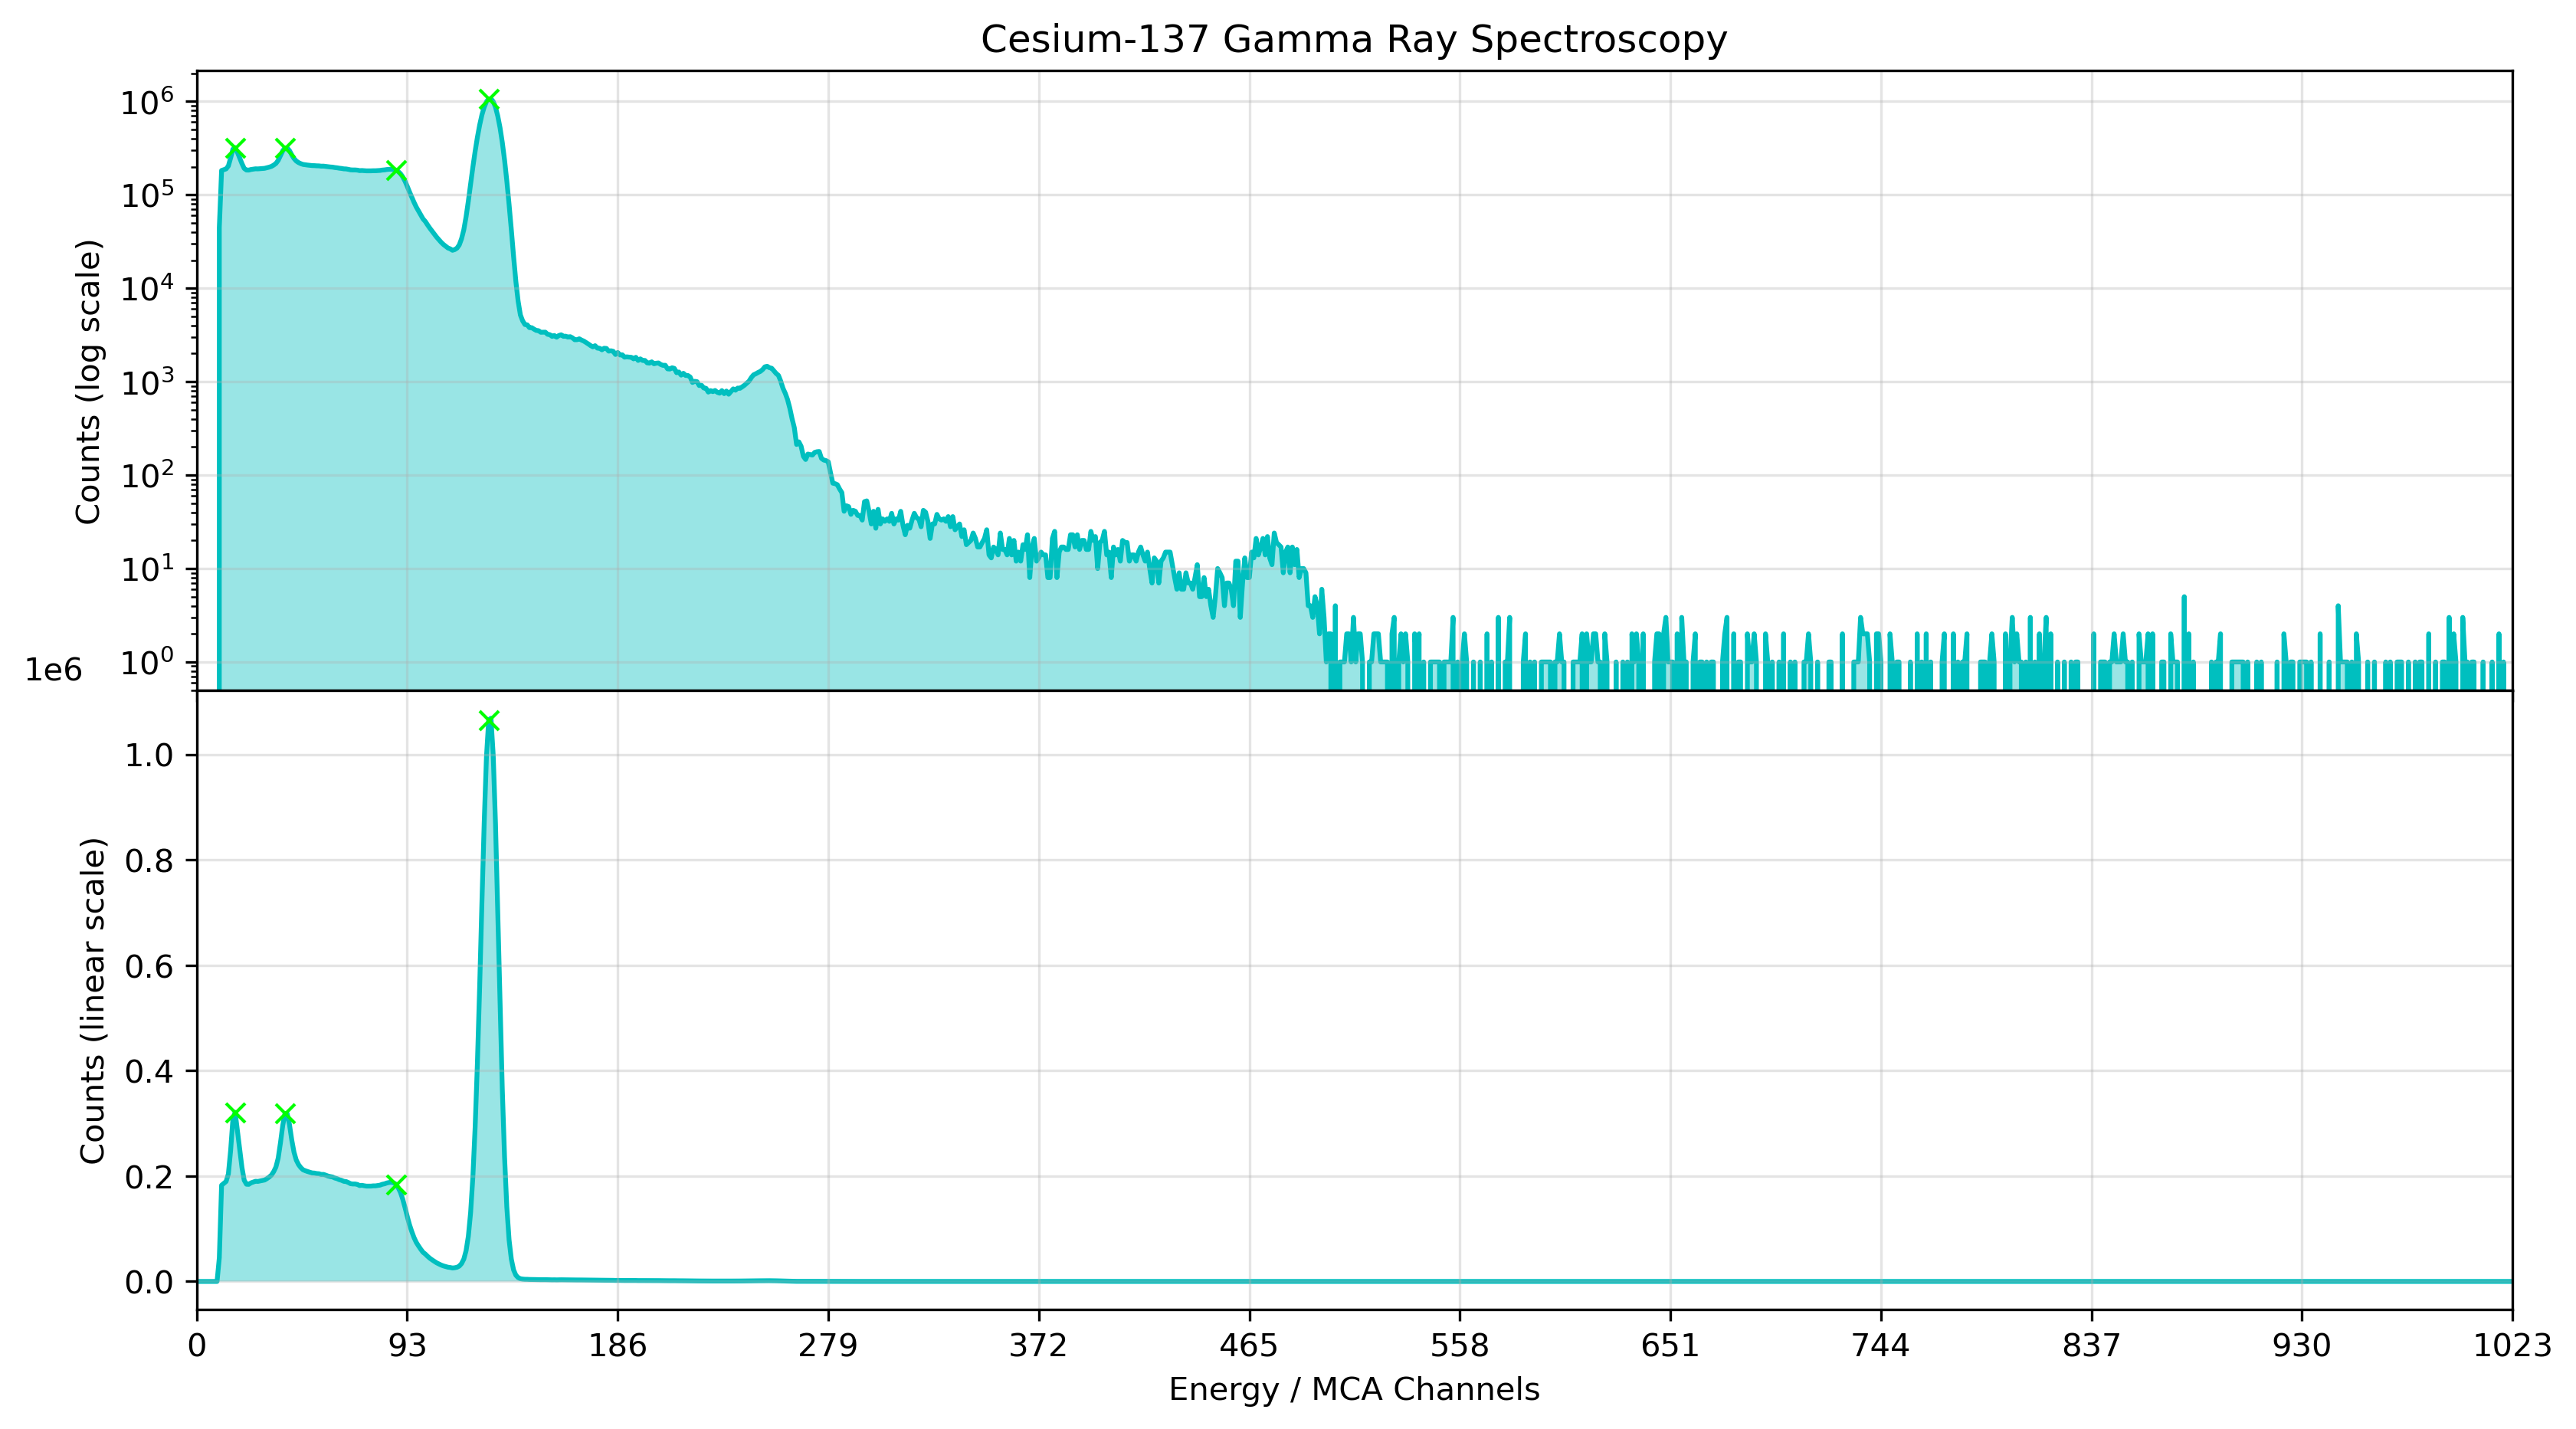
\includegraphics[width=0.98\linewidth]{figs/fig7a.png}
    \end{subfigure}
    \begin{subfigure}{0.98\linewidth}
        \centering
        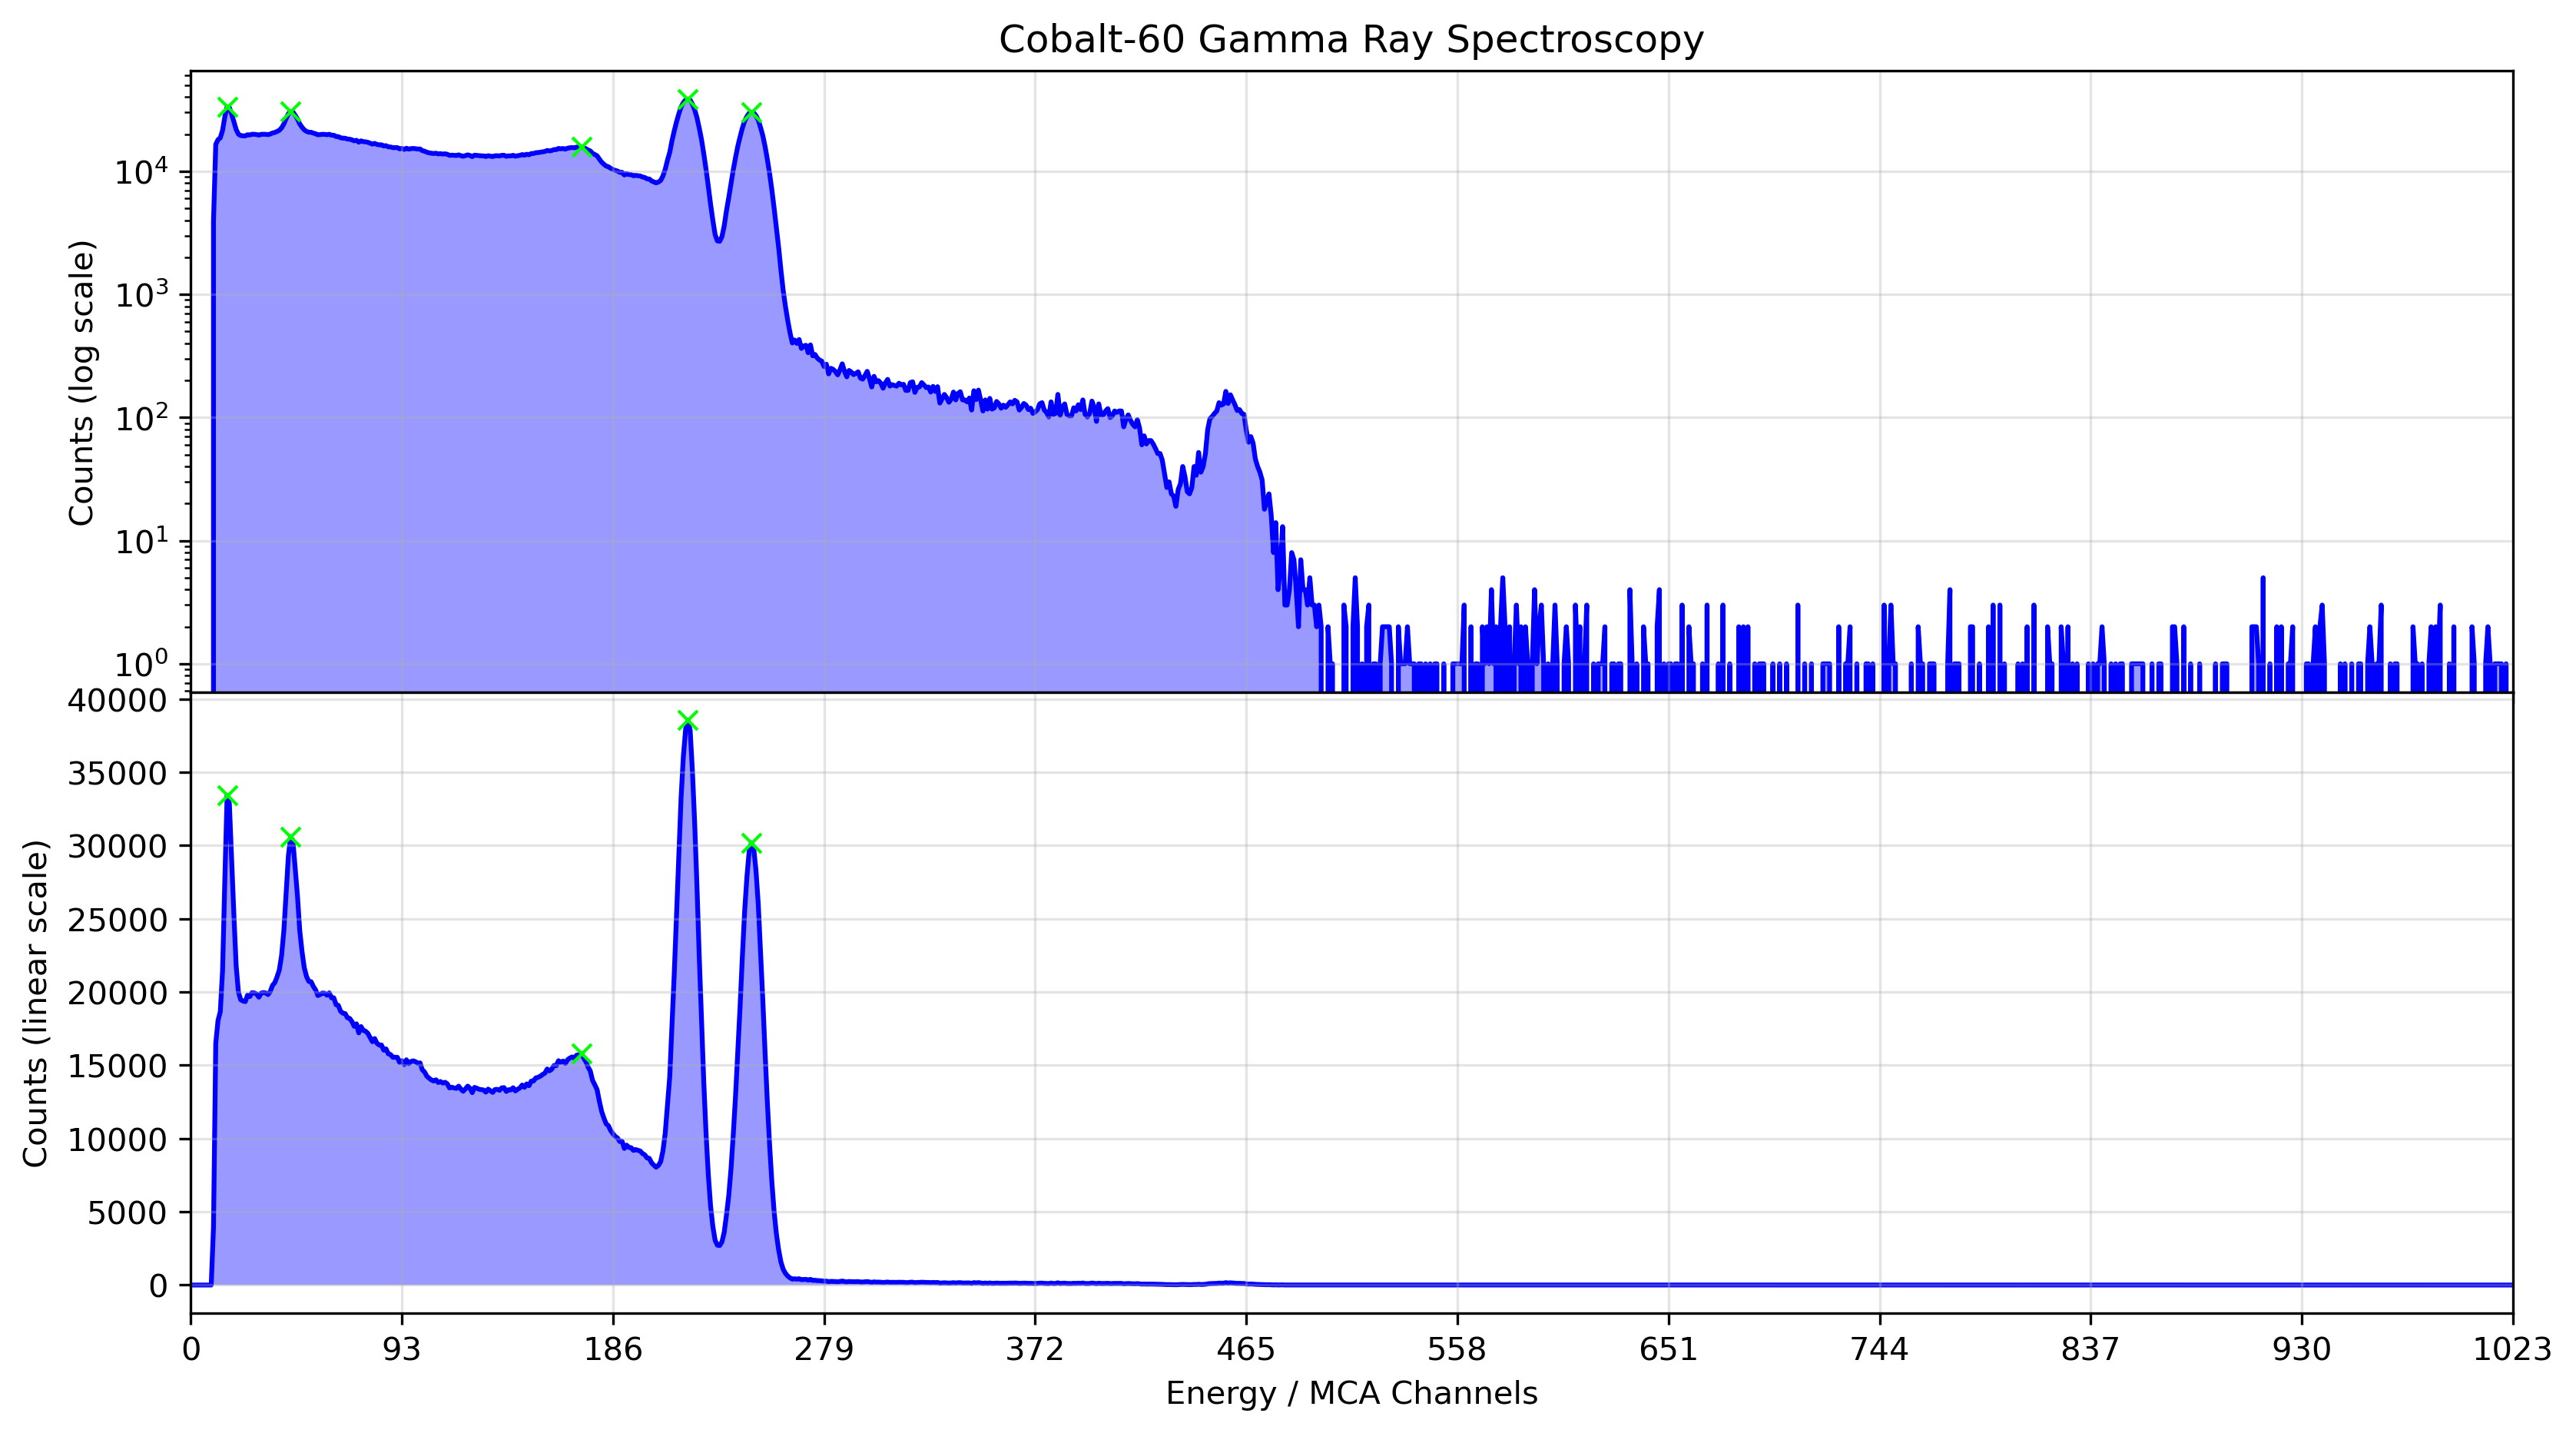
\includegraphics[width=0.98\linewidth]{figs/fig7b.png}
    \end{subfigure}
    \caption{
        Calibration gamma ray spectra of Cs-137 and Co-60. Green markers represent peaks found.
    }
\end{figure}
\begin{multicols}{2}
\noindent
unknown.
This paper decides to showcases a few of these opportunities via two forms:
(1) identification of an unlabeled (and therefore unknown) radiation sample found
within the laboratory; and
(2) Gaussian curve fitting for various known identifiable peaks for Na-22.
\begin{figure}[H]
    \centering
    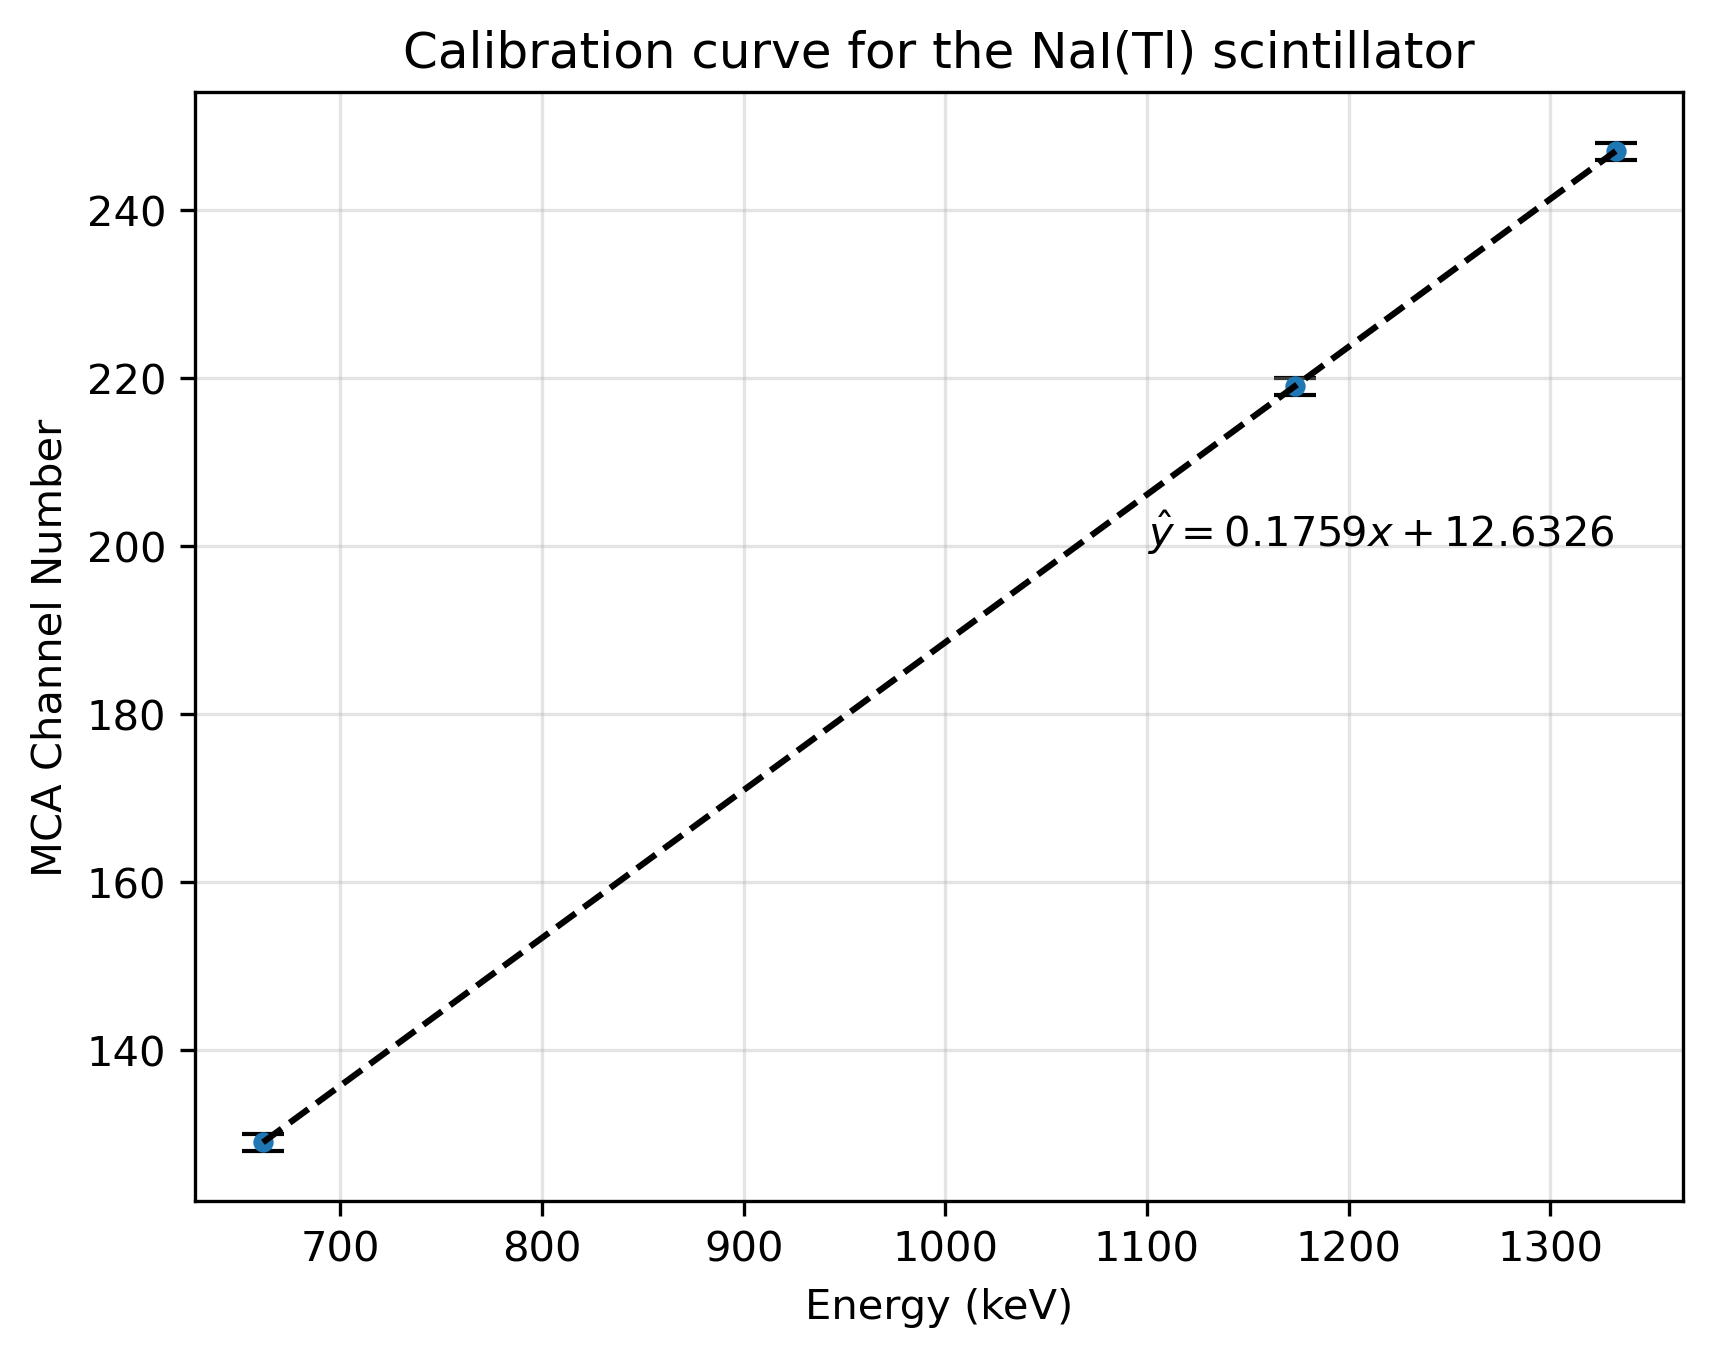
\includegraphics[width=0.98\linewidth]{figs/fig8.png}
    \caption{
        Calibration curve constructed using weighted linear least-squares fitting
        with known photopeak energy levels and experimentally determined photopeak
        position channel numbers.
    }
\end{figure}
\noindent
\subsubsection{Sample Identification}
\textbf{Figure 9} shows the gamma ray spectrum of said unlabeled radiation sample
found within the laboratory. It is at this point worth mentioning the probable
order of peak type appearances in order of having the least of energy to the
most: (1) X-rays; (2) annihilation; (3) backscatter; (4) Compton edge;
and (5) photoelectric. Not all sample may have the first two type of peaks,
as \textbf{Figure 7} showed that Cs-137 and Co-60 likely do not have 
annihilation peaks (it will be shown soon that Na-22 has one, which its count
outweighs the rest of the type of peaks). By that note,
typically then the highest peak would represent the photopeak, and given known
photopeak energy levels from various radiation sources this unknown radiation sample
can be identified.

From the determined channel number 132 as the position of the photopeak,
the predictive line fit model converts this number to approximately 35.850 keV.
From references, this result aligns with the lowest listed photopeak energy level,
35.5 keV, which belongs to Antimony-125 (Sb-125) [\textcolor{red}{?}].
A percent error calculation can be carried out between these two values,
but it is more notable to mention that the overestimation in converted energy level
is due to the position of the found photopeak position (notice how it is marked
slightly to the right of the peak in \textbf{Figure 9}), and in considering this
explanation, it is then well-supported to identify the unknown sample as Sb-125.

\subsubsection{Gaussian Curve Fitting}
\textbf{Figure 10} shows the gamma ray spectroscopy of Na-22.
Six peaks can be identified as, from left to right, X-ray lines (two of them),
the annihilation curve, backscatter, Compton edge, and a photopeak. 
If these peaks are isolated (usually by an ROI finder) at the center of the
found peak location channel number, a statistic method known as \textit{Markov
Chain Monte Carlo (MCMC)} may be carried out to probabilistically fit the most
ideal Gaussian curve to the data out of various sample runs. This can be done through
another open-sourced Python package (\texttt{pymc}), which allows users to build
Bayesian models to fit using MCMC.

\textbf{Figure 11} shows the result of the MCMC method for fitting Gaussian curves.
It can be seen that for the X-ray peaks, the model performs poorly, but is likely
explained to be due to the noise to opposite sides of each peak, incorrectly
shifting the prediction curves towards the noise. For the rest of the curves, however,
it can be qualitatively assessed to be good fits for the measurement points gathered.
It is mostly surprising that the model was able to fit the Compton edge well,
for it can be seen from \textbf{Figure 10} that its peak also has elevated counts
toward one side of its curve (like the X-rays).

The result of this analysis technique is incredibly useful for the capabilities of
being able to find some values for the \textit{true} parameters of a peak energy level
from experimental measurements through the robust methods of counting statistics.
\newpage

\end{multicols}
\begin{figure}[H]
    \centering
    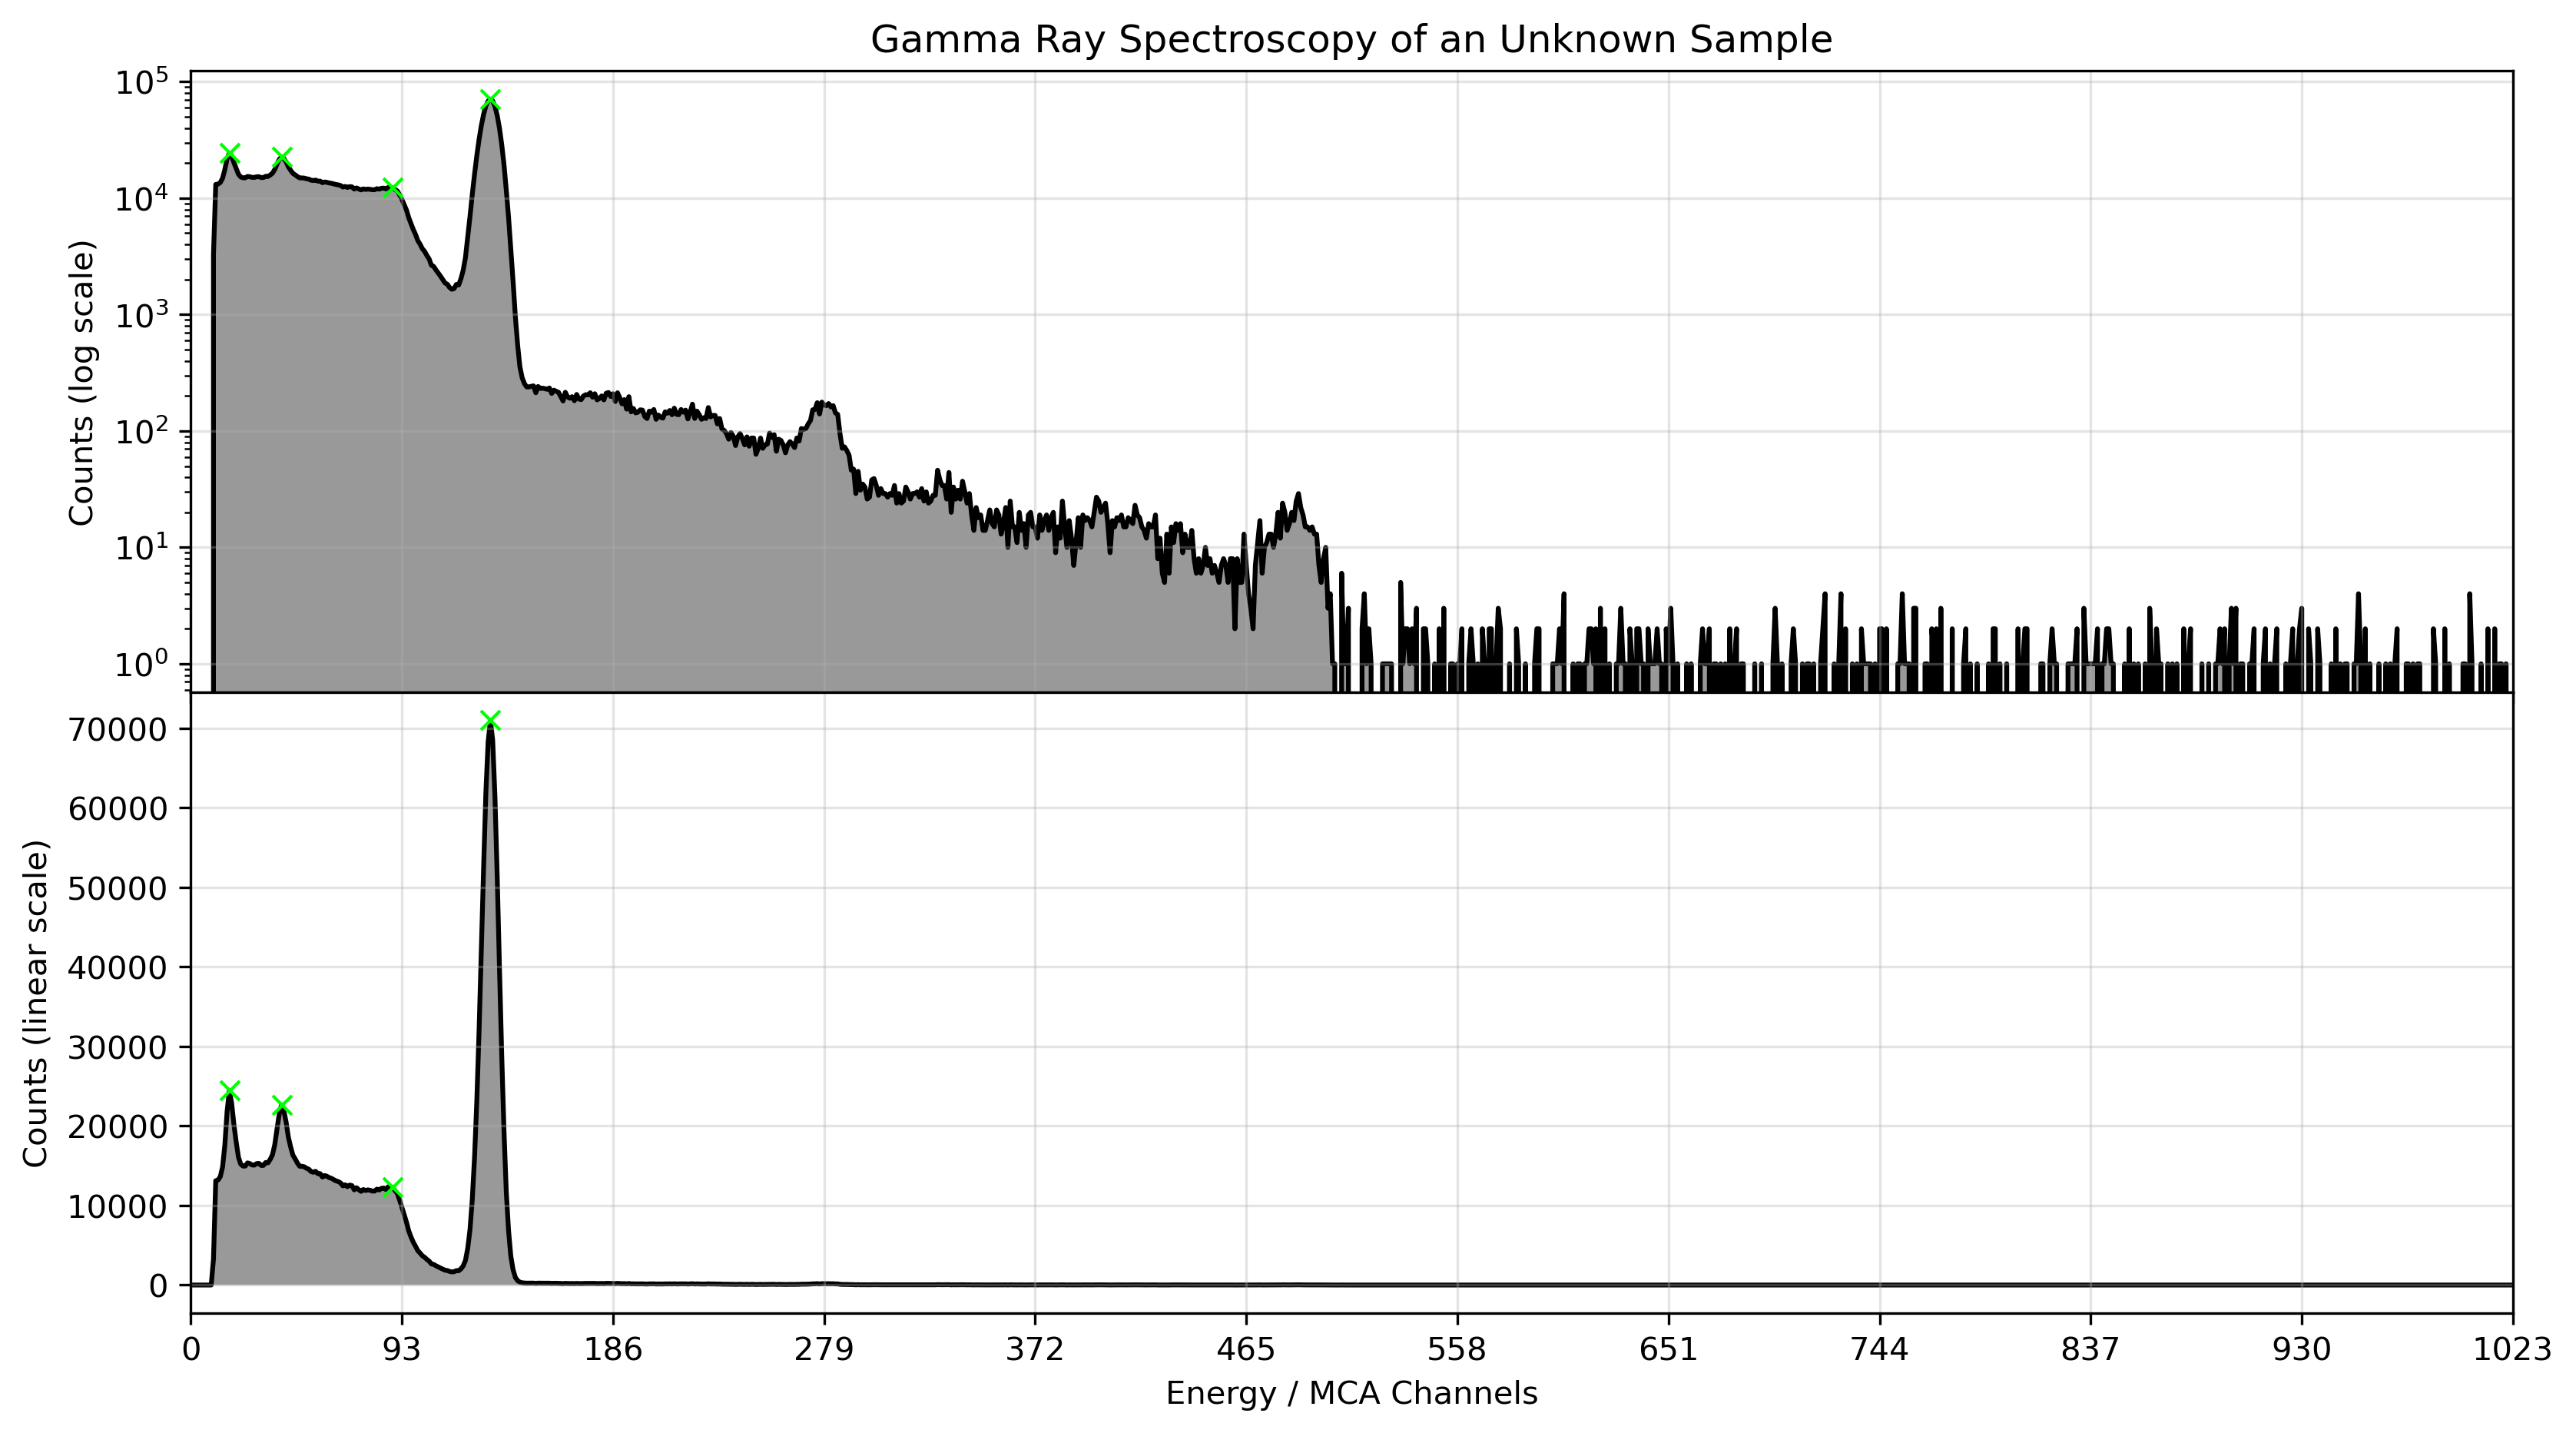
\includegraphics[width=0.98\linewidth]{figs/fig9.png}
    \caption{
        Gamma ray spectroscopy of an unlabeled radiation sample.
    }
\end{figure}
\begin{figure}[H]
    \centering
    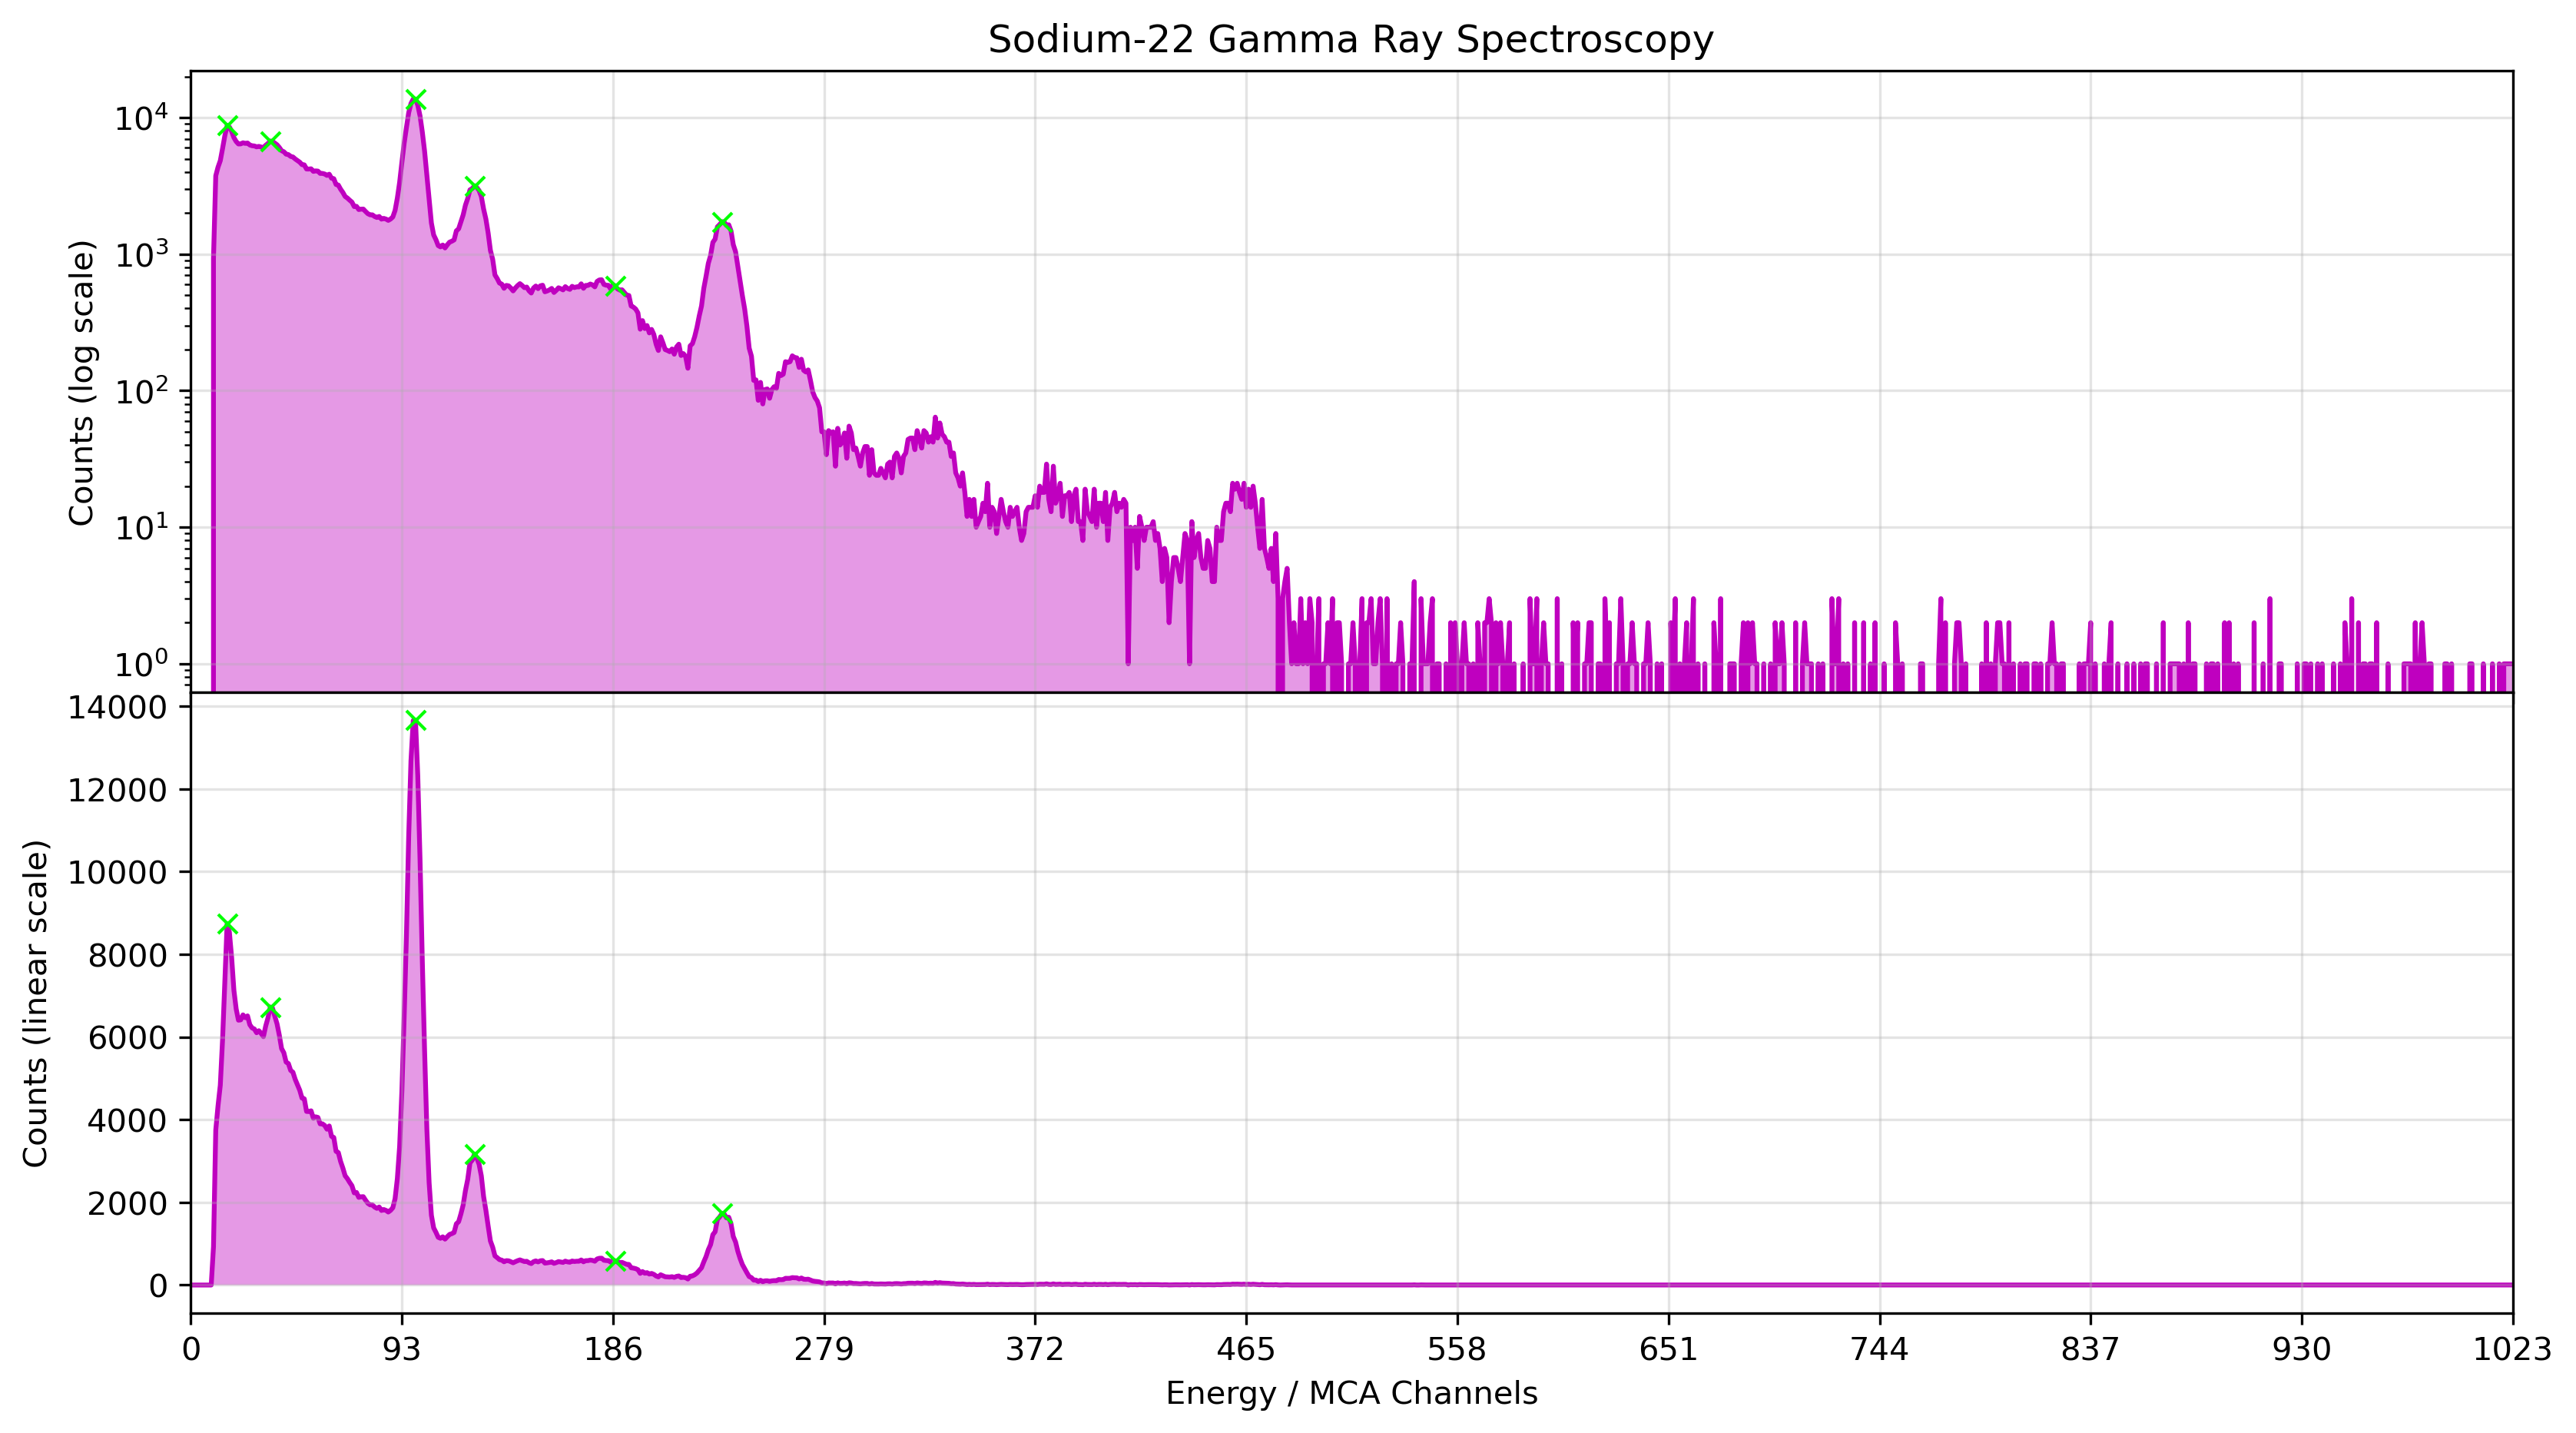
\includegraphics[width=0.98\linewidth]{figs/fig10.png}
    \caption{
        Gamma ray spectroscopy of Na-22.
    }
\end{figure}
\newpage
\begin{figure}[H]
    \centering
    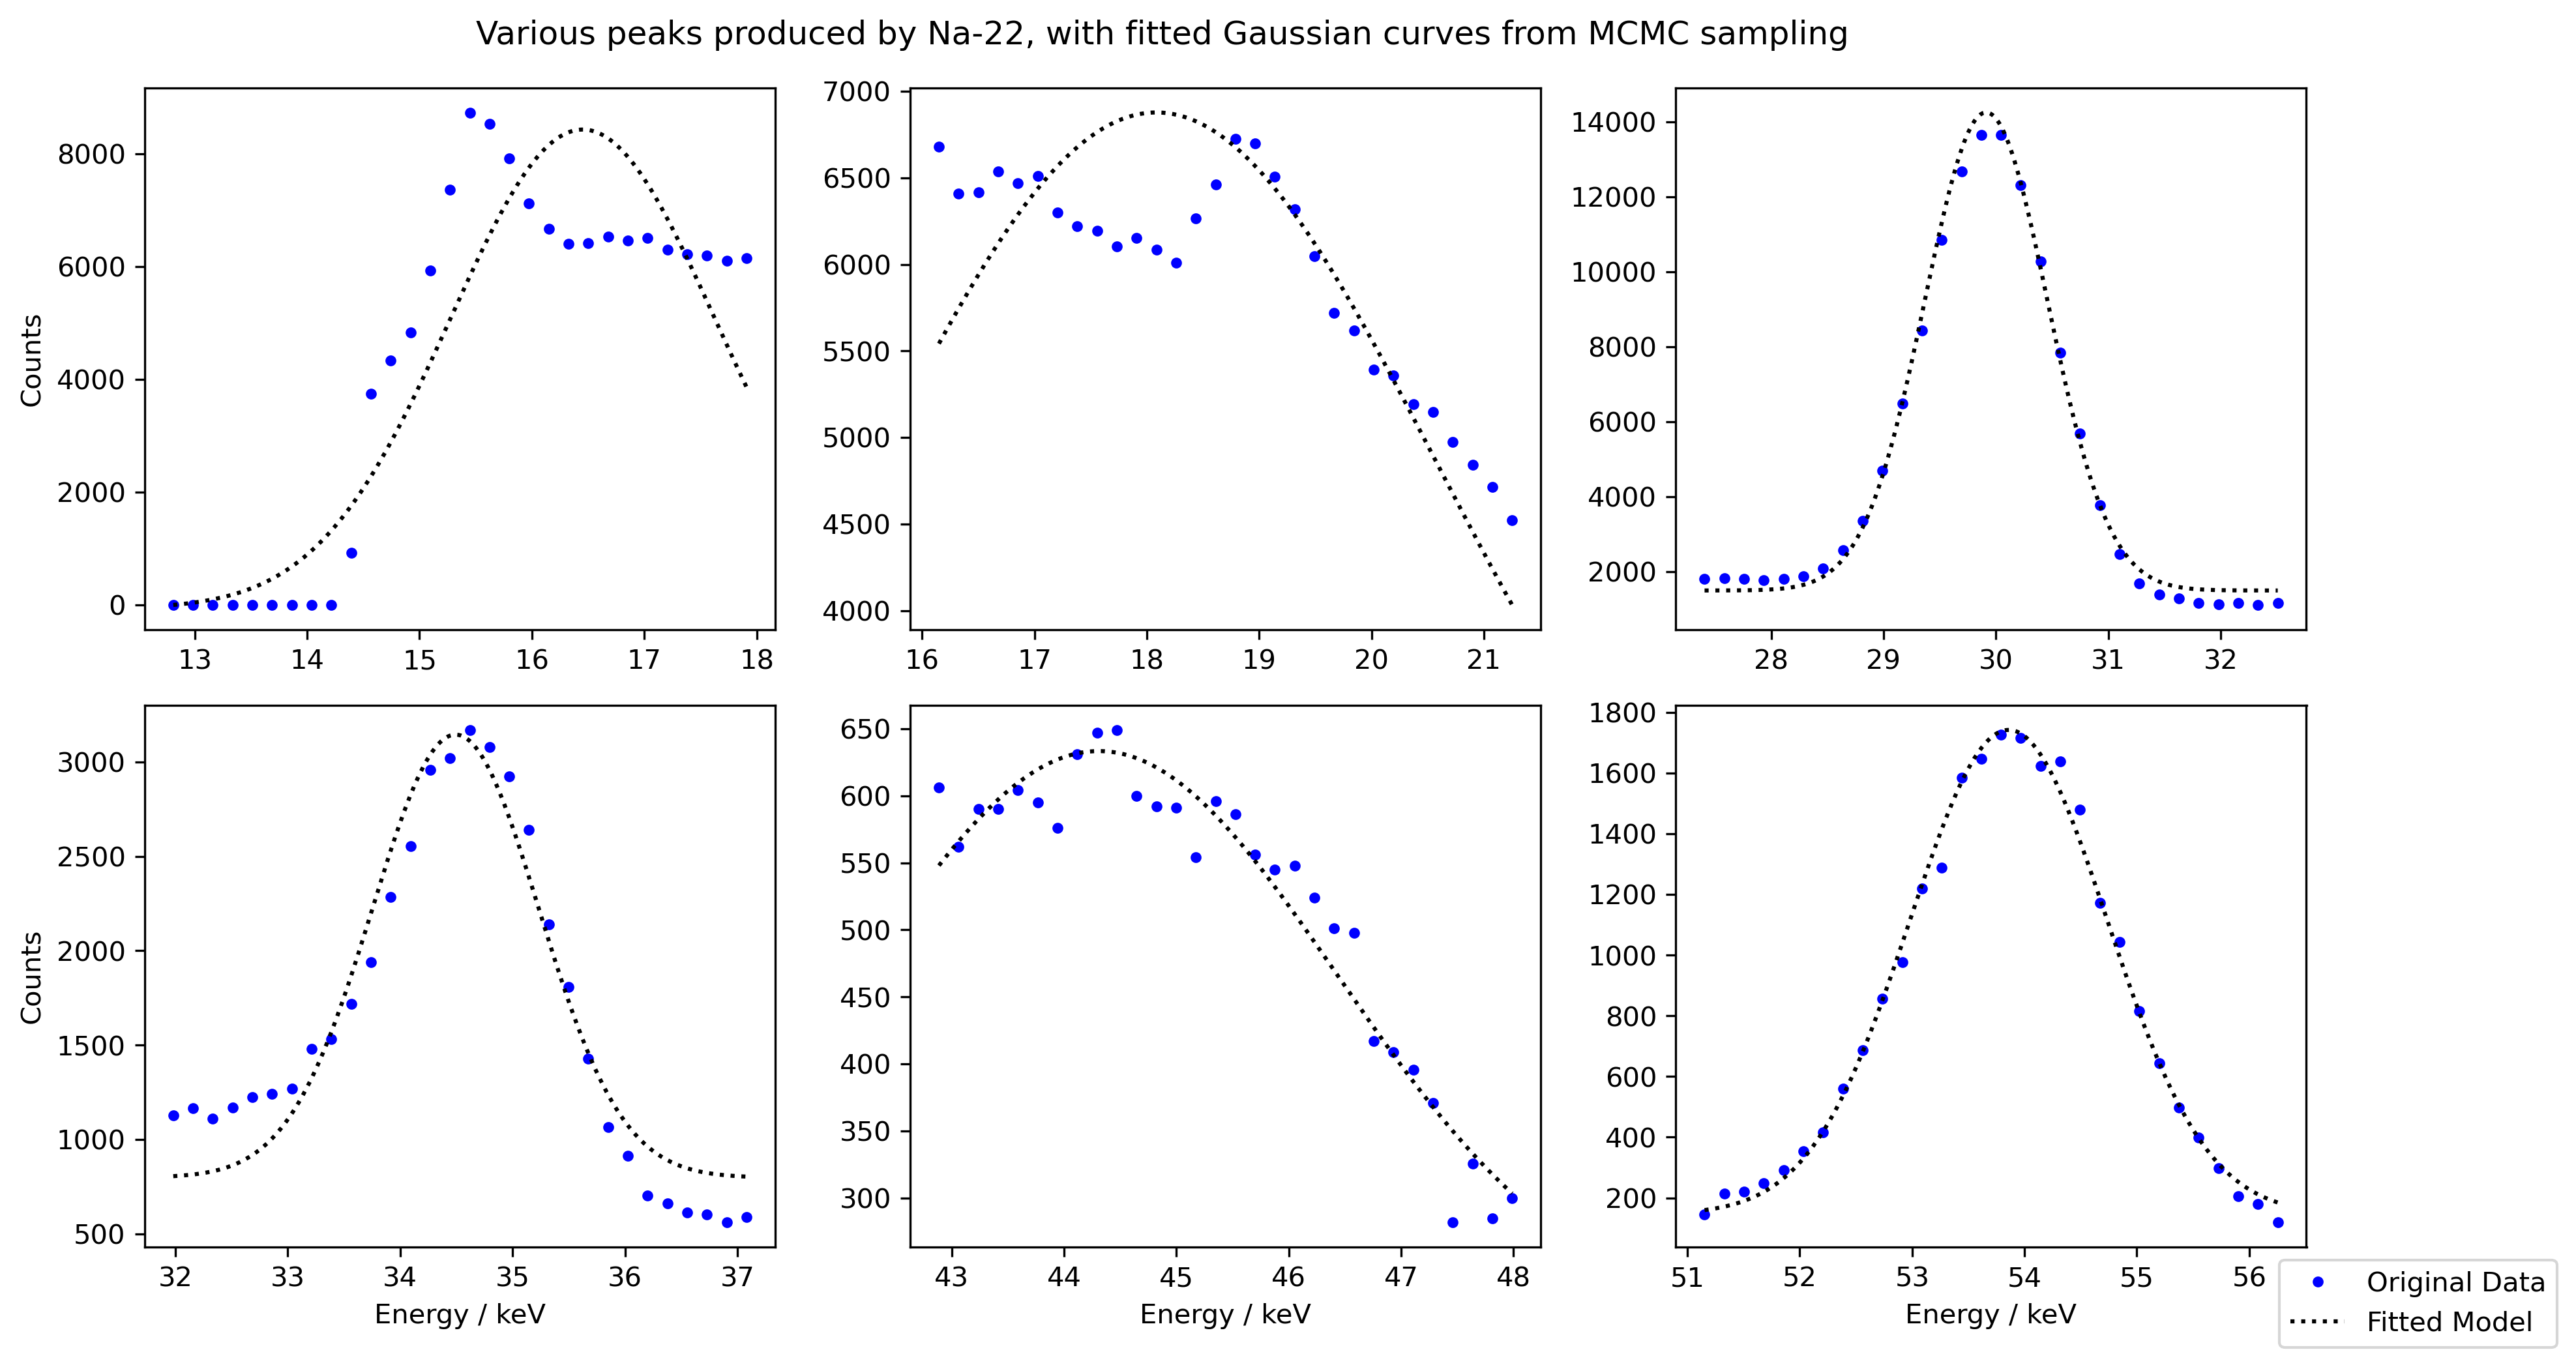
\includegraphics[width=0.98\linewidth]{figs/fig11.png}
    \caption{
        Gaussian curve fitting of six known peaks of Na-22 from \texttt{pymc}'s
        sampling using MCMC methods and Bayesian statistics.
    }
\end{figure}

%%%%%%%%%%%%%%
% References %
%%%%%%%%%%%%%%
\newpage

\subsection*{References}
\begin{enumerate}[label={[\arabic*]}]
    \item \label{sec:1} Nuclear Security \& Safeguards Education Portal, ``01-Basic Radiation Detection: Introduction to Radiation Detection'', \textit{YouTube} (2017), \url{https://youtu.be/y3UYdRJWacU?si=eN2ugshwfnOtzByx}
    \item \label{sec:2} Nuclear Security \& Safeguards Education Portal, ``21-Basic Radiation Detection: Gamma ray spectroscopy, part 1'', \textit{YouTube} (2017), \url{https://youtu.be/y3UYdRJWacU?si=eN2ugshwfnOtzByx}
    \item \label{sec:3} Francesco Sciacca, Photoelectric effect, \textit{Radiopedia} (Last revised on 29 Oct. 2024), \url{https://radiopaedia.org/articles/photoelectric-effect}
    \item \label{sec:4} Francesco Sciacca, Compton effect, \textit{Radiopedia} (Last revised on 29 Oct. 2024), \url{https://radiopaedia.org/articles/compton-effect}
    \item \label{sec:5} Raymond Chieng, Pair production, \textit{Radiopedia} (Last revised on 16 Jun. 2023), \url{https://radiopaedia.org/articles/pair-production}
    \item \label{sec:6} Nuclear Security \& Safeguards Education Portal, ``23-Basic Radiation Detection: Gamma: Scintillation Detectors'', \textit{YouTube} (2017), \url{https://www.youtube.com/watch?v=_IqxMYmZe6s}
\end{enumerate}

%%%%%%%%%%%%%%
% Appendices %
%%%%%%%%%%%%%%
\newpage

\subsection*{Appendix A: Derivation of the Compton Scattering Formula}
\begin{enumerate}
    % \item Begin with the Law of Conservation of Energy for the Compton effect
    % between a photon and an electron (essentially) at rest:
    % $$E_\gamma + E_0 = E_\gamma^\prime + E_e$$
    % where $E_\gamma$ is the initial kinetic energy of the photon,
    % $E_0$ is the rest energy of the electron,
    % $E_\gamma^\prime$ is the final kinetic energy of the photon,
    % and $E_e$ is the recoil energy of the electron.
    
    % \item Substitute the initial and final energy states of the electron
    % with the mass-energy equivalency formula, $E=mc^2$, to get
    % $$E_\gamma + m_ec^2 = E_\gamma^\prime + m_ec^2 + K\!E$$
    % where $m_e$ is the mass of the electron ($9.1094\times10^{-31}$ kg).
    % This can be simplified:
    % \begin{gather*}
    %     E_\gamma + \cancel{m_ec^2} = E_\gamma^\prime + \cancel{m_ec^2} + K\!E \\
    %     E_\gamma = E_\gamma^\prime + K\!E
    % \end{gather*}
    % and $K\!E$ can be isolated
    % $$K\!E = E_\gamma - E_\gamma^\prime$$

    % \item By definition, the energy of a photon ray is $E=hf$, so
    % substituting the corresponding energy states at the right-hand side
    % yields
    % $$K\!E=hf-hf^\prime$$
    % where $h$ is Planck's constant and $f$ is the wave frequency.
    % Use the frequency-wavelength relationship $c=\lambda f$ to furthermore
    % express the equation as
    % $$K\!E=\frac{hc}{\lambda}-\frac{hc}{\lambda^\prime}$$

    % \item Next, algebraic work to express $K\!E$ in terms of $\Delta\lambda\equiv\lambda^\prime-\lambda$
    % difference in wavelength so we may use the Compton Shift Formula:
    % \begin{align*}
    %     K\!E &= hc\qty(\frac{1}{\lambda}-\frac{1}{\lambda^\prime}) \\
    %     &= hc\qty(\frac{\lambda^\prime}{\lambda\lambda^\prime}-\frac{\lambda}{\lambda\lambda^\prime}) \\
    %     &= hc\qty(\frac{\lambda^\prime-\lambda}{\lambda\lambda^\prime}) \\
    %     &= hc\qty(\frac{\Delta\lambda}{\lambda\lambda^\prime})
    % \end{align*}

    % \item Group the terms into two overall fractions
    % $$K\!E = \qty(\frac{hc}{\lambda^\prime})\qty(\frac{\Delta\lambda}{\lambda})$$
    % and bring over the $\dfrac{\Delta\lambda}{\lambda}$ term over to the left-hand side via
    % multiplying both sides with its reciprocal
    % $$K\!E\qty(\frac{\lambda}{\Delta\lambda})=\frac{hc}{\lambda'}$$

    % \item \textit{Ansatz}: we may notice that $\frac{\Delta\lambda}{\lambda}$
    % is a ratio made up of the wavelength states of the photon,
    % with $K\!E$ as its coefficient. Assume that this is $E_\gamma^\prime$.
    
    %%%%%%%%%%%%%%%%%%%%%%%%%%%%%%%%%%%%%%%%%%%%%%%%%%%%%%%%%%%%%%%%%%%%%%%%%%%%%%%%%%%%%%%%%%%%%%%%%%%%%
    % ok in hindsight this entire step up to this point was just redundant; could have started here.... %
    %%%%%%%%%%%%%%%%%%%%%%%%%%%%%%%%%%%%%%%%%%%%%%%%%%%%%%%%%%%%%%%%%%%%%%%%%%%%%%%%%%%%%%%%%%%%%%%%%%%%%

    \item We are interested in expressing a formula for the final kinetic energy
    of a photon in terms of its initial kinetic energy before and after the Compton Effect.
    Begin with the final kinetic energy of a photon and the definition of photon
    energy
    $$E_\gamma'=hf'$$
    where $h$ is Planck's constant and $f$ is the wave frequency.
    Use the frequency-wavelength relationship $c=\lambda f$ to express
    the equation as
    $$E_\gamma'=\frac{hc}{\lambda'}$$
    
    \item At the right-hand side, introduce $\lambda$ in the denominator via
    addition and subtraction
    $$E_\lambda'=\frac{hc}{\lambda'+\lambda-\lambda}$$
    define $\Delta\lambda\equiv\lambda'-\lambda$ the wavelength difference
    between the two energy states
    $$E_\gamma'=\frac{hc}{\Delta\lambda+\lambda}$$

    \item We would like at the end to be able to express in terms of energy
    via $E=hf$, so the $hc$ term at the right must be algebraically expressed
    as $hf$ instead. Divide the numerator and denominator respectively
    with $\lambda$
    $$E_\gamma'=\dfrac{\dfrac{hc}{\lambda}}{\dfrac{\Delta\lambda+\lambda}{\lambda}}$$
    the numerator is just the initial kinetic energy of the photon $E_\gamma$.
    Linearly divide $\lambda$ in the denominator
    $$E_\gamma'=\dfrac{E_\gamma}{1+\dfrac{\Delta\lambda}{\lambda}}$$

    \item Use the Compton Shift formula $\Delta\lambda=\lambda_c\big(1-\cos(\theta)\big)$
    $$E_\gamma'=\dfrac{E_\gamma}{1+\dfrac{\lambda_c}{\lambda}\big(1-\cos(\theta)\big)}$$
    where $\lambda_c$ is the Compton wavelength of an electron.
    Express $\lambda_c$ in terms of fundamental constants $\lambda_c=\dfrac{h}{m_ec}$,
    where $m_e$ is the mass of the electron
    $$E_\gamma'=\dfrac{E_\gamma}{1+\dfrac{h}{\lambda}\dfrac{1}{m_ec}\big(1-\cos(\theta)\big)}$$

    \item Multiply $\dfrac{h}{\lambda}$ by $c$ and divide $\dfrac{1}{m_ec}$ by $c$
    (this does not change the overall equation since $\dfrac{c}{c}=1$)
    $$E_\gamma'=\dfrac{E_\gamma}{1+\dfrac{hc}{\lambda}\dfrac{1}{m_ec^2}\big(1-\cos(\theta)\big)}$$
    where $\dfrac{hc}{\lambda}$ the initial kinetic energy of the photon $E_\gamma$ appears again
    $$E_\gamma'=\dfrac{E_\gamma}{1+\dfrac{1}{m_ec^2}E_\gamma\big(1-\cos(\theta)\big)}$$

    \item The rest energy of an electron is given by the mass-energy equivalence relation $E_e=m_ec^2$.
    Use fundamental constant values $m_e=9.1094\times10^{-31}$ kg, $c=2.9979\times10^8\;\mathrm{\sfrac{m}{s}}$
    and the conversion factor $1\;\mathrm{MeV}/c=5.344\times10^{-22}\;\mathrm{kg\cdot\sfrac{m}{s}}$ to finally get
    $$E_\gamma'=\dfrac{E_\gamma}{1+1.96\;\mathrm{MeV}\;E_\gamma\big(1-\cos(\theta)\big)}$$
    where 1.956859003 MeV $\approx$ 1.96 MeV was approximated.
    
    \hfill$\blacksquare$
\end{enumerate}


\end{document}